\documentclass{uvamscse}

\usepackage{listings}

\lstdefinelanguage{sdf}{%
  numbers=none,
  morekeywords={module,imports,exports,sorts,context,lexical,free,syntax,==,=,+,-,left,cons,prefer,avoid,bracket},
  columns=flexible,
  morestring=[b]",
  basicstyle=\footnotesize\mdseries,
  literate={->}{{\,\,$\to$\,\,}}1
}

\lstdefinelanguage{dcg}{%
  numbers=none,
  morekeywords={},
  morestring=[b]",
  basicstyle=\footnotesize\mdseries,
  columns=flexible,
}

\lstdefinelanguage{prolog},
  literate={:-}{{\,$\Leftarrow$\,\,}}1 {-->}{{$\to$\,}}1
}

\lstdefinestyle{mono}{
  basicstyle=\footnotesize\ttfamily
}

\lstset{%
  frame=none,
  xleftmargin=2pt,
  stepnumber=1,
  numbers=left,
  numbersep=7pt,
  numberstyle=\ttfamily\scriptsize\color[gray]{0.3},
  belowcaptionskip=\bigskipamount,
  captionpos=b,
%  escapeinside={*'}{'*},
  % language=fl,
  tabsize=2,
  emphstyle={\bf},
  stringstyle=\itshape,
  showspaces=false,
  keywordstyle=\bfseries\rmfamily,
  columns=flexible,
  basicstyle=\small\mdseries,
  showstringspaces=false,
}

\newcommand{\cmd}[1]{\texttt{$\backslash$#1}}

\usepackage[toc,acronym,nogroupskip]{glossaries}
\usepackage{url}

\usepackage{graphicx}
\graphicspath{ {figures/} }

% ====== Listing Setup =======
% \usepackage{color}
% \usepackage{listings}
% \definecolor{javared}{rgb}{0.6,0,0} % for strings
% \definecolor{javagreen}{rgb}{0.25,0.5,0.35} % comments
% \definecolor{javapurple}{rgb}{0.5,0,0.35} % keywords
% \definecolor{javadocblue}{rgb}{0.25,0.35,0.75} % javadoc
 
% \lstset{language=Java,
% 	basicstyle=\ttfamily,
% 	keywordstyle=\color{javapurple}\bfseries,
% 	stringstyle=\color{javared},
% 	commentstyle=\color{javagreen},
% 	morecomment=[s][\color{javadocblue}]{/**}{*/},
% 	keywordstyle={[2]\color{red}\bf},
% 	numbers=left,
% 	numberstyle=\tiny\color{black},
% 	stepnumber=1,
% 	numbersep=10pt,
% 	tabsize=2,
% 	showspaces=false,
% 	showstringspaces=false
% }

% ====== Glossaries setup =======
\makeglossaries
\newcommand{\ac}[1]{\gls{#1}}
\newcommand{\acs}[1]{\acrshort{#1}}
\newcommand{\acp}[1]{\glspl{#1}}

\newacronym{oop}{OOP}{Object Oriented Programming}
\newacronym{aop}{AOP}{Aspect Oriented Programming}

%%%%%%%%%%%%%%%%%%%%%%%%%%%%%%%%%%%%%%%%%%%%%%%%%%%%%%%%%%%%%%%%%%%%%%%%%%%%%%%
% Title
%%%%%%%%%%%%%%%%%%%%%%%%%%%%%%%%%%%%%%%%%%%%%%%%%%%%%%%%%%%%%%%%%%%%%%%%%%%%%%%
\title{Taming Aspects with Managed Data }
% \coverpic[100pt]{figures/terminal.png}
% \subtitle{A Thesis Template Leading by Example}
\date{Summer 2016}

\author{Theologos A. Zacharopoulos}
\authemail{theol.zacharopoulos@cwi.nl}
\supervisor{Tijs van der Storm}
\host{Centrum Wiskunde \& Informatica, \url{http://www.cwi.nl}}

\begin{document}

\abstract{
	% CCC
	% AOP
	% Managed data
}

\maketitle

%%%%%%%%%%%%%%%%%%%%%%%%%%%%%%%%%%%%%%%%%%%%%%%%%%%%%%%%%%%%%%%%%%%%%%%%%%%%%%%
% Chapters
%%%%%%%%%%%%%%%%%%%%%%%%%%%%%%%%%%%%%%%%%%%%%%%%%%%%%%%%%%%%%%%%%%%%%%%%%%%%%%%
%%%%%%%%%%%%%%%%%%%%%%%%%%%%%%%%%%%%%%%%%%%%%%%%%%%%%%%%%%%%%%%%%%%%%%%%%%%%%%%
% Chapter: Introduction
%%%%%%%%%%%%%%%%%%%%%%%%%%%%%%%%%%%%%%%%%%%%%%%%%%%%%%%%%%%%%%%%%%%%%%%%%%%%%%%
\chapter{Introduction}\label{Introduction}
\ac{ccc} is a problem for which the classic programming techniques can not tackle with sufficiently. 
This results in scattered and tangled code, which affects the system's modularity and it's ease of maintenance and evolution. 
Since \ac{oop} and \ac{pp} techniques can not solve this problem, \ac{aop} presented \cite{kiczales1997aspect} in order to
provide a solution by introducing the notion of \textit{aspects}.

\ac{aop} results in a modular and \textit{single-responsibility} design whose properties must be implemented as \textit{components} (cleanly encapsulated procedure) and \textit{aspects} (not clearly encapsulated procedure), both separate concepts that are combined for the result through a process called \textit{weaving}. 
However, relying on \ac{aop}, paradoxically, does not improve the evolution of a project even with the modularity that it provides 
since it introduces tight coupling between the aspects and the application. 
As a result the way to tackle with this problem we need a more sophisticated and expressing crosscut language.
Consequently, \ac{ccc} could be handled in a higher level of the language such as the data structuring and management mechanisms.

Managed data \cite{loh2012managed} allows programmers to take control of important aspects of data as reusable modules. 
Using managed data a developer can build \textit{data managers} that handle the fundamental data manipulation primitives 
that are usually hard-coded in the programming language, by introducing custom data manipulation mechanisms. 
Managed data have been researched and implemented under the Enso project\footnote{\label{enso}\url{http://enso-lang.org/}}, which is developed in Ruby\footnote{\label{ruby}\url{https://www.ruby-lang.org/en/}} (a dynamic programming language) using Ruby’s reflection capabilities. 
Furthermore, managed data are considered less able to be supported in static languages directly which makes it more challenging for 
this thesis since it is going to be implemented in Java.
In this thesis I am going to use the Java reflection capabilities to implement managed data and focus on specific aspects and design patterns implementations using the data managers concept of managed data. 

%%%%%%%%%%%%%%%%%%%%%%%%%%%%%%%%%%%%%%%%%%%%%%%%%%%%%%%%%%%%%%%%%%%%%%%%%%%%%%%
\section{Initial Study}\label{Initial Study}
% TODO: more
In their study on managed data, Loh et al. \cite{loh2012managed} present an implementation of managed data
in Ruby and they use as a case study a web development framework from the Enso project to reuse database management and 
access control mechanisms across different data definitions.

This thesis is an extension of their work; we implement managed data in Java (a static programming language) using the Java reflection API\footnote{\url{https://docs.oracle.com/javase/tutorial/reflect/}} and dynamic proxies\footnote{\url{https://docs.oracle.com/javase/8/docs/api/java/lang/reflect/Proxy.html}}. 
Although proxies in static programming languages can not implement the full range of managed data \cite{loh2012managed}. 
Java provides a strong implementation of the meta-object protocol \cite{kiczales1991art}, which can be used though the Java Reflection API \cite{forman2004java}. 
Additionally, this project will focus on aspects and will provide a solution to the \ac{ccc} problem by using managed data.

%%%%%%%%%%%%%%%%%%%%%%%%%%%%%%%%%%%%%%%%%%%%%%%%%%%%%%%%%%%%%%%%%%%%%%%%%%%%%%%
\section{Problem statement}\label{Problem statement}

The problem we study regards the \ac{ccc} that are scattered around the application, resulting to a hard to maintain system 
by tangling implementation logic and concerns code together.
Even though, \ac{aop} provides new modularization mechanisms, which should result in easier evolving software, 
it delivers solutions that are as hard and sometimes even harder to evolve than before \cite{tourwe2003existence}. 
The problem lays on the aspects, which have to include a crosscut description of all places in the application where this code yields an influence. 
Thus, the aspects are tightly coupled to the application and this greatly affects the evolvability of the overall system. 

Additionally, Friedrich Steimann \cite{steimann2005domain} argues that modeling languages are not aspect ready. 
The problem that arises is located at the level of software modeling. 
More specifically, in \textit{roles modeling}, whereas in \ac{oop} roles are tied to the collaborations,
collaborations rely on interactions of objects, and aspects on the other hand are typically defined independently of one another. 

Furthermore, in terms of order, it has been observed that aspects are not elements of the domain, they describe the order rather than the domain. 
Finally, aspects invariably express non-functional requirements, but if the non-functional requirements are not elements of domain models then neither are aspects.

In order to solve the aforementioned problems, we implement manage data, lifting the data management up to the application.

%%%%%%%%%%%%%%%%%%%%%%%%%%%%%%%%%%%%%%%%%%%%%%%%%%%%%%%%%%%%%%%%%%%%%%%%%%%%%%%
\subsection{Problem Analysis}\label{Problem Analysis}
% TODO: FOCUS HERE 
% An analysis of the problem: where does it occur and how, how often, and what are the consequences? An important part is also to scope the research: what aspects are included and what aspects are deliberately left out, and why?

%%%%%%%%%%%%%%%%%%%%%%%%%%%%%%%%%%%%%%%%%%%%%%%%%%%%%%%%%%%%%%%%%%%%%%%%%%%%%%%
\subsection{Research Questions}\label{Research Questions}
Managed data has not been practically implemented in a static language before, therefore my first research questions states 
``Can managed data be implemented in a static language like Java?''. 
Based in the previous argumentation about the relevance of \ac{aop} and the solutions that managed data can provide in \ac{ccc}, my second research question is ``Can managed data solve \ac{ccc} and to what extend does it improve the software evolution problems that \ac{aop} introduces in a modular solution?''. 
Finally by using a software showcase, the JHotDraw framework, as well as its \ac{aop} implementation AJHotDraw \cite{marinajhotdraw}, 
I am going to evaluate the implementation of managed data on an inventory of aspects and design patterns. 
As a result the third research question states ``To what extent can managed data tame an inventory of aspects and design patterns in the JHotDraw framework, in contrast with the original and the AOP implementation.''

%%%%%%%%%%%%%%%%%%%%%%%%%%%%%%%%%%%%%%%%%%%%%%%%%%%%%%%%%%%%%%%%%%%%%%%%%%%%%%%
\subsection{Solution Outline}\label{Solution Outline}
Our solution is consisted of an implementation of managed data in Java. 
This framework can be used by applications in order to deal with \ac{ccc}.

To validate our hypotheses we are going to implement managed data in Java using the Java Reflection API and Dynamic Proxies. 
More specifically we are going to use Java interfaces for \textit{schemas} and dynamic proxies for \textit{data managers}. 
Furthermore, we are going to provide as a proof of concept the examples given in \cite{loh2012managed} but this time developed in Java. As mentioned in \cite{loh2012managed} to stack data managers I am going to use the Decorator Pattern \cite{gamma1995design}. 

In order to prove that managed data solves the problems that \ac{aop} introduces, we are going to implement an inventory of the following aspects and design patterns from JHotDraw using data managers:
\begin{description}
  \item[The Observer Pattern,] which as presented in literature \cite{tourwe2003existence} \cite{hannemann2005role} \cite{marin2005approach}, is by nature not modularized and the scatters pattern code through the classes. 
  This pattern is considered as a difficult case because it is used a lot in the original JHotDraw source code but with multiple variations, thus it is difficult to extract an abstract version.

  \item[The Singleton Pattern,] which as presented \cite{hannemann2005role} \cite{hannemann2002design}, it can easily be abstracted as an aspect and replace the \ac{oop} usage in JHotDraw. 

  \item[The Template Method,] which as presented \cite{hannemann2005role} \cite{hannemann2002design}, it scatters code by introducing roles such as those of \textit{AbstractClass} and \textit{ConcreteClass}.

  \item[The Undo aspect,] which is analyzed extensively \cite{marin2004refactoring} and a solution is provided by AJHotDraw. 
  More specifically, this aspect consists of aspect-oriented refactoring of the \textit{Command} pattern with \textit{Undo} actions.
\end{description}

This inventory is implemented using data managers that have modularity as a main characteristic and is been evaluated in a new JHotDraw implementation. 
We compare those aspects with the original version of JHotDraw, and the aspect version, AJHotDraw. 
Since our solution is a refactoring of the JHotDraw framework we need a way to ensure the behavioral equivalence between the original and the refactored solution \cite{fowler2009refactoring}. 
However, JHotDraw comes with no tests. 
Thus, we use the TestJHotDraw, which is a subproject of the AJHotDraw development team, and it is developed in order to contribute to a gradual and safe adoption of aspect-oriented techniques in existing applications and allow for a better assessment of aspect orientation.
Since we use our JHotDraw implementation for the functional evaluation of our solution, we can use the presented criteria \cite{hannemann2002design}, which are \textit{Locality},\textit{Re-usability}, \textit{Composition Transparency}, and \textit{(Un)pluggability}, in order to present metrics of our solution. 

%%%%%%%%%%%%%%%%%%%%%%%%%%%%%%%%%%%%%%%%%%%%%%%%%%%%%%%%%%%%%%%%%%%%%%%%%%%%%%%
\subsection{Research Method}\label{Research Method}
The answers for the research questions have been extracted from the background material, in our Java managed data implementation and an evaluation of our implementation in an existing use case system the JHotDraw.

\begin{description}

  \item[Managed data implementation in a static language.]
  In order to answer the question if managed data could be implemented in a static language, we've implemented managed data in Java 
  using Java's reflection capabilities\footnote{\url{https://docs.oracle.com/javase/tutorial/reflect/}}, using Java interfaces 
  for schemas definition and dynamic proxies\footnote{\url{https://docs.oracle.com/javase/8/docs/api/java/lang/reflect/Proxy.html}}
  for the data managers. An extensive presentation of the implementation is given in Chapter \ref{Implementation}.

  \item[Use case implementation and evaluation.] In order to argue about the contribution of our implementation and managed data for aspects handling in general, we've used an use case application (JHotDraw) which is considered as a good design use case for \ac{oop}, along with it's \ac{aop} implementation (AJHotDraw). Using these application as references we've implemented our own version of JHotDraw using managed data to tame some of it's aspects, the results are presented extensively in Chapter \ref{Evaluation}.

\end{description}	

%%%%%%%%%%%%%%%%%%%%%%%%%%%%%%%%%%%%%%%%%%%%%%%%%%%%%%%%%%%%%%%%%%%%%%%%%%%%%%%
\section{Contributions}\label{Contributions}

\begin{description}
  \item[Contribution 1: Managed data implementation in Java.]
  Our first contribution with this thesis is the implementation of managed data in a static language like Java.
  Managed data implemented as an internal \ac{dsl} in Java, using interfaces for schema definitions and dynamic proxies
  for the data managers.

  \item[Contribution 2: Managed data Java framework.]
  The final deliverable is a Java library with which the developer can define and implement aspects as reusable modules
and integrate them with an application without mixing the business logic with concern logic.
More specifically, the schemas and the data managers have to be defined by the developer, as well as any additional
functionality that may needed to be integrated to the patterns or roles of the application.

  \item[Contribution 3: Managed data Evaluation in JHotDraw.]
  We implemented a new version of the JHotDraw application using our framework in order to evaluated our \ac{ccc} solution.
  More specifically, we focused on the \textit{Undo} concern, which is scattered around the implementation of the JHotDraw.

  \item[Contribution 4: JHotDraw implementation results assessment and comparison with AJHotDraw.]
  Finally, we present the results of our evaluation and we compare them we another implementation of the JHotDraw which 
  implements aspects using \ac{aop} and the AspectJ language, the AJHotDraw.

\end{description}

%%%%%%%%%%%%%%%%%%%%%%%%%%%%%%%%%%%%%%%%%%%%%%%%%%%%%%%%%%%%%%%%%%%%%%%%%%%%%%%
\section{Related Work}\label{Related Work}
In this section we discuss the related work of research that inspired this thesis. 
More specifically, we discuss points that we followed and points that we've tried to improve as well as the reason of doing it.

\begin{description}

  \item[Meta-Object Protocol]~\\
  Managed data can be implemented using reflection and the \ac{mop}. 
  The authors of Enso \cite{loh2012managed} implemented it in Ruby using reflection and the \textbf{method\_missing} mechanism. 
  In other languages (such as Java, JavaScript or C\#) that support dynamic proxies, they can be used for the managed data implementation, which is the way we've implemented it.
  The \ac{mop} \cite{kiczales1991art} was first implemented for simple \ac{oop} capabilities of the Lisp language in order to satisfy some developer demands including compatibility, extensibility and developers experimentation. 
  The idea was that the languages have been designed to be viewed as black box abstractions without giving the programmers the control over semantics or the implementation of those abstractions. 
  \ac{mop} opens up those abstractions to the programmer so he can adjust aspects of the implementation strategy. 
  Providing an open implementation can be advantageous in wide range of high-level languages and that \ac{mop} technology is a powerful tool for providing that power to the programmer \cite{kiczales1991art}. 
  Furthermore, \ac{mop} provides flexibility to the programmer because as a language becomes more and more high level and it's expressive power becomes more and more focused, the ability to cleanly integrate something outside the language's scope becomes more and more difficult. 
  Thus, both \ac{mop} and managed data allow the programmer to be able to control the interpretation of structure and behavior in a program.
  However, \ac{mop} focuses on behavior of the objects and classes, while in managed data focus on the data management only.
  One could conclude that managed data is a subset of the \ac{mop} approach since managed data have a more narrow scope.


  \item[Adaptive Object Model]~\\
  Managed data \cite{loh2012managed} is closely related to the \ac{aom}. \ac{aom} \cite{yoder2002adaptive} is an architectural style that emphasizes flexibility and runtime dynamic configuration. 
  Architectures that are designed to adapt at runtime to new user requirements by retrieving descriptive information that can be interpreted at runtime, are sometimes called a ``reflective architecture'' or a ``meta architecture''. 
  An \ac{aom} system, is a system that represents classes, attributes, relationships, and behavior as metadata, something that is closely related to the managed data.
  However, on one hand \ac{aom} style is more general than the managed data since it is described at a very high level as a pattern language. Additionally, it covers business rules and user interfaces, in addition to data management. 
  On the other hand, \ac{aom} does not discuss issues of integration with programming languages, the representation of data schemas, or of bootstrapping, which are central characteristics of managed data. \ac{aom} is also presented as a technique for implementing business systems, not as a general programming or data abstraction technique \cite{loh2012managed}.

  \item[Model Driven Software Development]~\\
  \ac{mdsd} refers to a software development method which generates code from defined models. 
  The model represent abstract data that consisted of the structure and properties definition of an entity.
  The idea of the model in \ac{mdsd} is closely related to the \textit{schemas} in managed data.
  Similarly to the model definition, schemas define the structure, the properties and any meta-data that describe an entity
  following by a code generation that adds functionality to that entity for it's manipulation.

  \item[The Enso Language]~\\
  Enso project\footnote{\url{http://enso-lang.org/}} is the first implementation of managed data, 
  it is open source\footnote{\url{https://github.com/enso-lang/enso}} and is used for EnsoWeb, a web framework written with managed data.
  Although Enso is implemented in Ruby, which is a dynamic language, the source code was a informative place to start for our static implementation in Java. 
  The structure of Enso was an inspiration of our implementation even though some parts have changed completely in order to follow our needs and support of Java's static system.
  Additionally, examples presented in Enso, are also implemented in our case and are presented in the Appendix \ref{Example Application}.

  \item[Aspect Oriented Programming]~\\
  Although \ac{aop} is not directly connected to managed data, it allows a mechanism that is relative easy to be supported in managed data.
  This mechanism consist of the \textit{weaving} of aspect code in specific join points. 
  The way to support this mechanism in managed data it is through data managers, which it is the main topic of this thesis and 
  is going to presented deeply in the following chapters.

\end{description}

%%%%%%%%%%%%%%%%%%%%%%%%%%%%%%%%%%%%%%%%%%%%%%%%%%%%%%%%%%%%%%%%%%%%%%%%%%%%%%%
\section{Document Outline}\label{Document Outline}
In this section we outline the structure of this thesis. 
In Chapter \ref{Background} we introduce the background, focusing on the concepts, which the reader must be familiarizes with 
in order to follow the next chapters.
In Chapter \ref{Theory} a basic theory is presented, which is going to be used a a reference for our implementation.
In Chapter \ref{Implementation} the implementation is demonstrated and analyzed, providing explanation of our issues 
and implementation details.
Next, in Chapter \ref{Evaluation} an evaluation of our implementation is presented, by applying it in JHotDraw. 
Additionally, some metrics, claims and results are presented.
Finally, a conclusion is given in Chapter \ref{Conclusion} along with some further work in \ref{Further Work}.


% !TEX root = ../thesis.tex

%%%%%%%%%%%%%%%%%%%%%%%%%%%%%%%%%%%%%%%%%%%%%%%%%%%%%%%%%%%%%%%%%%%%%%%%%%%%%%%
% Chapter: Background
%%%%%%%%%%%%%%%%%%%%%%%%%%%%%%%%%%%%%%%%%%%%%%%%%%%%%%%%%%%%%%%%%%%%%%%%%%%%%%%
\chapter{Background}\label{Background}

%%%%%%%%%%%%%%%%%%%%%%%%%%%%%%%%%%%%%%%%%%%%%%%%%%%%%%%%%%%%%%%%%%%%%%%%%%%%%%%
% Section: CCC
%%%%%%%%%%%%%%%%%%%%%%%%%%%%%%%%%%%%%%%%%%%%%%%%%%%%%%%%%%%%%%%%%%%%%%%%%%%%%%%
\section{Cross Cutting Concerns}\label{Cross Cutting Concerns}
There is a significant research in software engineering that focuses on the importance of software modularity. 
The number of advantages of modular systems is outrageous, with maybe the most significant the extensibility and evolution of a system \cite{parnas1972criteria}.

However, during the development of a system there is a number of concerns that they have to be considered and implemented into the system. 
In order to follow the modularity principles, those concerns have to be implemented in a separate modules, this way the program will be extensible and its evolution easier.
Nonetheless, many of those concerns can not fit into the existing modular mechanisms of any of the existing programming paradigms including both \ac{oop} and \ac{pp}. 
In those cases, the concerns are scattered through the modules of the system, resulting to scattered and tangled code. 
Those concerns called \acrlong{ccc} \cite{hannemann2005role}.
\ac{ccc} considered a serious issue for the evolution of a system and the effects of tangled and scattered code disastrous for a system's extensibility.

The reason is that the code which is related to a concern, is scattered in multiple modules, while the concern code is tangled with the different modules logic. 
Thus, this results to a system which does not follow the \textit{Single Responsibility Principle} and consequently the system will be hard to maintain.

Some examples of those \ac{ccc} are persistence, caching, logging, error handling \cite{lippert2000study}, access control and many more. 
Additionally, some design patterns scatter ``design pattern code'' thought the application, such as the \textit{Observer Pattern}, \textit{template Pattern}, \textit{command Pattern} etc. \cite{hannemann2002design} \cite{marin2004refactoring}.

In order to solve this problem we need a way to refactor and transform the non-modularized \ac{ccc} into a modular \textit{aspect}.
Refactorings of \ac{ccc} should replace all the scattered and tangled code of a concern with an equivalent module \cite{hannemann2005role}, which in \ac{aop} it is called \textit{aspect} \cite{kiczales1997aspect}.

%%%%%%%%%%%%%%%%%%%%%%%%%%%%%%%%%%%%%%%%%%%%%%%%%%%%%%%%%%%%%%%%%%%%%%%%%%%%%%%
% Section: AOP
%%%%%%%%%%%%%%%%%%%%%%%%%%%%%%%%%%%%%%%%%%%%%%%%%%%%%%%%%%%%%%%%%%%%%%%%%%%%%%%
\section{Aspect Oriented Programming}\label{Aspect Oriented Programming}

Kiczales et al. present \cite{kiczales1997aspect} by using an example of a very simple image processing application. 
In that system, and in general, whenever two properties being programmed must compose differently and yet be coordinated (in the example filters and loop-fusion), they \textbf{crosscut} each other.
Because general purposes languages provide only one composition mechanism, which mechanisms lead to complexity and tangling, the programmer must do the co-composition manually. 
According to their theory, an system's property can be either a \textit{component}, if it \textbf{can} be cleanly encapsulated in a generalized procedure, or an \textit{aspect}, if it \textbf{can not} be cleanly encapsulated in a generalized procedure. 
\ac{aop} supports the programmer in cleanly separating components and aspects from each other by providing mechanisms that makes possible to abstract and compose them together when producing the whole system. 
This is in contrast to common programming paradigms, \ac{oop} and \ac{pp}, that allow programmers in only separating the \text-it{components} from each other but crosscut the concerns.

However, implementing \ac{aop} programs is not that easy since several tools are needed in order to succeed it. 
More specifically, a general purpose language needs only a language, a \textit{compiler} and a \textit{program} written in the language that implements the application.
In case of an \ac{aop} based implementation, a program consists of a \textit{component language}, in which the components are programmed, one or more \textit{aspect languages}, in which the aspects are programmed, an aspect \textit{weaver} for the combined languages, a \textit{component program} that implements the components using the component language and finally, one or more \textit{aspect programs} that implement the aspects using the aspect languages.
Additionally, an essential function of the aspect weaver is the concept of join points, which are those elements of the component language semantics that the aspect programs coordinate with. 

%%%%%%%%%%%%%%%%%%%%%%%%%%%%%%%%%%%%%%%%%%%%%%%%%%%%%%%%%%%%%%%%%%%%%%%%%%%%%%%
\subsection{AspectJ}\label{AspectJ}
There is a some significant work in the area of aspect oriented languages but one the most important contribution is the AspectJ\footnote{\url{https://eclipse.org/aspectj/}} project, which is a simple and practical aspect-oriented extension to Java and it has been introduced by Kiczales et al. \cite{kiczales2001overview}.
The authors of AspectJ provide examples of programs developed in AspectJ and show that by using it, \ac{ccc} can be implemented in clear form, which in other general purpose languages would lead to tangled and scattered code. 
AspectJ was developed as a compatible extension to Java so that it would facilitate adoption by current Java programmers. 
The compatibility lays on upward compatibility, platform compatibility, tool compatibility, and programmer compatibility. One of the most important characteristic of AspectJ is that it is not a \ac{dsl} but a general purpose language that uses Java's static type system.
All of the above properties are those that we target for our managed data implementation as well.

%%%%%%%%%%%%%%%%%%%%%%%%%%%%%%%%%%%%%%%%%%%%%%%%%%%%%%%%%%%%%%%%%%%%%%%%%%%%%%%
\subsection{Design Patterns in \acrlong{aop}}\label{Design Patterns in Aspect Oriented Programming}

Hannemann et al. present a showcase of \ac{aop} \cite{hannemann2002design} in which they conduct an aspect-oriented implementation of the Gang of Four design patterns \cite{gamma1995design} in AspectJ, in which 17 out of 23 cases show modularity improvements.
Even though design patterns offer flexible solutions to common software problems, those patterns involve crosscutting structures between roles and classes / objects. 
There are several problems that the \ac{oop} design patterns introduce in respect of \ac{ccc}, and specifically in cases when one object plays multiple roles, many objects play one role, or an object play roles in multiple patterns \cite{sullivan2002advanced} (design pattern composition).

The problem lays on the way a design pattern influences the structure of the system and its implementation, pattern implementations are often tailored to the instance of use, and this often leads them to disappear into the code and lose their modularity \cite{hannemann2002design}. Even worst, in case of multiple patterns used in a system (pattern overlay and pattern composition), it can become difficult to trace particular instances of a design pattern. 
Composition creates large clusters of mutually dependent classes\cite{sullivan2002advanced}, and some design patterns explicitly use other patterns in their solution.

\subsubsection{Observer pattern in \acrlong{aop}}\label{Observer pattern in Aspect Oriented Programming}
Hannemann et al. \cite{hannemann2002design} provide some example implementations of several design patterns, including the \textit{Observer Pattern} in which they focus on with a detailed implementation \ref{The Observer Pattern in JHotDraw}.
As they mention, in a observer pattern implementation, both the \textit{Subject} and the \textit{Observer} have to know about their roles and hence have ``pattern related code'' in them, consequently adding or removing code from a class, requires changes of code in that class. 

In their implementation \cite{hannemann2002design} of the observer pattern in AspectJ, they separate abstract aspects for: 

\begin{itemize}
	\item The \textit{Subject} and \textit{Observer} roles in classes.

	\item Maintenance of a mapping from \textit{Subjects} to \textit{Observers}.

	\item The trigger of \textit{Subjects} that update \textit{Observers}.
\end{itemize}

And concrete aspects for each instance of the pattern fills in the specific parts:
\begin{itemize}
	\item Which classes can be \textit{Subjects} and which \textit{Observers}.

	\item A set of changes on the \textit{Subjects} that triggers the \textit{Observers}.

	\item The specific means of updating each kind of \textit{Observer} when the update logic requires it.
\end{itemize}

\subsubsection{Modularity Properties}\label{Modularity Properties}
The modularity properties which this implementation relates are\cite{hannemann2002design}:

\begin{description}
	\item [Locality:] All the code that implements the \textit{Observer} pattern is in the abstract and concrete observer aspects, none of it is in the participant classes. 
	The participant classes are entirely free of the pattern context, and as a consequence there is no coupling between the participants.

	\item [Reusability:] The core pattern code is abstracted and reusable. 
	The abstract aspect can be reused and shared across multiple \textit{Observer} pattern instances.

	\item [Composition transparency:] Because a pattern participants implementation is not coupled to the pattern, if a \textit{Subject} or \textit{Observer} takes part in multiple observing relationships their code does not become more complicated and the pattern instances are not confused. 

	\item [(Un)pluggability:] Because \textit{Subjects} and \textit{Observers} don't need to be aware of their role in any pattern instance, it is possible to switch between using a pattern and not using it in the system. 
\end{description}

% TODO: Too much detail???
% \subsubsection{More design pattens in \acrlong{aop}}\label{More design pattens in Aspect Oriented Programming}
% Other patterns that are presented in the paper \cite{hannemann2002design} are clustered based on common features. 
% In case of the \textit{Composite}, \textit{Command}, \textit{Mediator}, \textit{Chain of responsibility}, the roles only used within pattern aspect. 
% More specifically, these patterns introduce roles that need no client-accessible interface and are only used within the pattern, e.g. in Composite pattern, to allow walking the tree structure inherent to the parents, the authors define facilities to have visitor traverse and/or change the structure. 

% There visitors are defined in the concrete aspect.
% The patterns \textit{Singleton}, \textit{Prototype}, \textit{Memento}, \textit{Iterator}, \textit{Flyweight} have aspects as object factories. 
% They administrate access to specific object instances. 
% All of them offer factory methods to clients and share a create-on-demand strategy. 
% The patterns are abstracted with code for the factory in the aspect. 
% Participants no longer need to have pattern code in them, the otherwise close coupling between an original object and its representation or accessors is removed from the participants.

% In case of the patterns \textit{Adapter}, \textit{Decorator}, \textit{Strategy}, \textit{Visitor} and \textit{Proxy}, using AspectJ the implementation of some patterns completely disappear because AspectJ language constructs implement them directly. This applies to these patterns in varying degrees. Next, the patterns \textit{Abstract Factory}, \textit{Factory Method}, \textit{Template Method}, \textit{Builder} and \textit{Bridge} can be implemented using multiple inheritance, AspectJ provides a solution to implement multiple inheritance in Java. The patterns \textit{State} and \textit{Interpreter} introduce high coupling between their participants. In the AspectJ implementations, parts of the scattered code can be modularized. Finally, the Facade pattern shows no benefit from AspectJ because there is no significant difference between the AspectJ and the Java implementation of this pattern. 

% As it has been presented above, Hannemann et al. \cite{hannemann2002design} evaluate their solutions by using the following criteria: \textit{Locality}, \textit{Reusability}, \textit{Composition Transparency}, and \textit{(Un)pluggability}.

In general an object or a class that is not coupled to its role in a pattern can be used in different contexts without modifications and the reusability of participants can be increased. 
The locality also means that existing classes can be incorporated into a pattern instance without the need to adapt them with extra effort, all the changes are made in the pattern instance. 
This makes the pattern implementations themselves relatively (un)pluggable. 
If we can reuse generalized pattern code and localize the code for a particular pattern instance, this can result in multiple instances of the same pattern in one application making easy to understand (composition transparency). 
This solves a common problem with having multiple instances of a design pattern in one application.

%%%%%%%%%%%%%%%%%%%%%%%%%%%%%%%%%%%%%%%%%%%%%%%%%%%%%%%%%%%%%%%%%%%%%%%%%%%%%%%
\subsection{Evolvability issues}\label{Aspect Oriented Programming Evolvability}
Since modularization and separation of concerns makes the evolution of an application a lot easier and \ac{aop} provides mechanisms for modularization and system decomposition, aspect-oriented programs should be easier to be evolved and maintained.
Paradoxically this is not the case \cite{tourwe2003existence} since \ac{aop} technologies deliver applications that are as hard, and sometimes even harder to than was the case before.

According to Tourwe et al. \cite{tourwe2003existence} the problem is that aspects have to include a crosscut description of all places in the application. 
Thus, it is much harder to make such crosscuts unaware to the application and most importantly to the rest of the modules. 
Additionally, current means for specifying concerns rely heavily in the existing structure of the application, therefore the aspects are tightly coupled to the application (and its structure) and of course this affects negatively the evolvability of a system since it makes it hard to change structurally.
As Tourwe \cite{tourwe2003existence} proposes, a solution for this problem would be the creation of a new, more sophisticated crosscut language. 
A language that enables the developer to discriminate between methods based on what they actually do instead of what they look like, in a more intentional way.
This is something that we tried to show in our thesis, a new language that implements \ac{ccc} in a modular way.

%%%%%%%%%%%%%%%%%%%%%%%%%%%%%%%%%%%%%%%%%%%%%%%%%%%%%%%%%%%%%%%%%%%%%%%%%%%%%%%
% Section: Managed Data 
%%%%%%%%%%%%%%%%%%%%%%%%%%%%%%%%%%%%%%%%%%%%%%%%%%%%%%%%%%%%%%%%%%%%%%%%%%%%%%%
\section{Managed Data}\label{Managed Data}
Managed data \cite{loh2012managed} is a data abstraction mechanism that allows the programmer to control the definition of the data and their manipulation mechanisms, additionally it provides a modular way to control aspects of data.
Managed data helps the programmer by giving them control over the structuring mechanism, which until now were predefined from the programming languages. 
The developers could not take control on them, but they could only to create data of those types.
Significant flexibility is provided since it lifts data management up to the application level by allowing the programmer to build data managers that handle the fundamental data manipulation primitives that are normally hard-coded into the programming language. 

Managed data has three essential components:

\begin{description}
	\item [Data description language,] that describe the desired structure and properties of data.
	\item [Data managers,] that enable creation and manipulation of instances of data.
	\item [Integration,] with a programming language to allow data created and manipulated.
\end{description}

In the traditional approach, the programming language includes a process and data definition mechanism, which are both predefined. 
However, with managed data, the data structuring mechanisms are defined by the programmer by interpretation of data definitions. 
Of course, since a data definition model is also data, it requires a meta-definition mechanism.

%%%%%%%%%%%%%%%%%%%%%%%%%%%%%%%%%%%%%%%%%%%%%%%%%%%%%%%%%%%%%%%%%%%%%%%%%%%%%%%
\subsection{Schemas}\label{Schemas}
The schemas are the way to describe the structure and the behavior of the data to be managed. 
They can be just a simple data description language which programmers can use to describe simple kind of data. 
For example Loh et al. \cite{loh2012managed} used Ruby hash for the data description on a simple example where the hash was an object that represented a mapping from values to values. 
However, a simple schema format like this can not be used to describe itself because it is not a record. 

A self-describing would allow schemas to be managed data themselves, thus we need a self-describing schema that can be used to describe schemas. 
A Schema-Schema(self-describing) is also managed data with its own data manager. 
This process is called \textit{Bootstrapping} and it is needed in order to ``jumpstart'' the process, this extends the benefits of programmable data structuring to their own implementation.
Schemas can be interpreted in many different ways to create different kinds of records based on the manipulation provided by the data managers.

%%%%%%%%%%%%%%%%%%%%%%%%%%%%%%%%%%%%%%%%%%%%%%%%%%%%%%%%%%%%%%%%%%%%%%%%%%%%%%%
\subsection{Data Managers}\label{Data Managers}
Data managers are the mechanisms that interpret \textit{schemas} with defined manipulation strategies set by the programmers. 
The input to a data manager is a schema, which describes the structure of the data to be managed.
Since the schema is only known dynamically the data managers must be able to determine the fields and methods of the managed data object dynamically as well.
In order to implement such operation we need a meta-programming mechanism that dynamically analyses the structure of a schema and applies the functionality of the data managers to it.
In their implementation Loh et al. \cite{loh2012managed} used the ``missing\_method'' implementation in order to succeed that.
In case of Java we will use reflection and dynamic proxies.

%%%%%%%%%%%%%%%%%%%%%%%%%%%%%%%%%%%%%%%%%%%%%%%%%%%%%%%%%%%%%%%%%%%%%%%%%%%%%%%
% Section: Reflection
%%%%%%%%%%%%%%%%%%%%%%%%%%%%%%%%%%%%%%%%%%%%%%%%%%%%%%%%%%%%%%%%%%%%%%%%%%%%%%%
\section{Java Reflection and Dynamic Proxies}\label{Java Reflection and Dynamic Proxies}
The Java programming language provides the programmer with a Reflection API\footnote{\url{https://docs.oracle.com/javase/tutorial/reflect/}} and with it offers the ability to examine or modify the runtime behavior of applications running in the \ac{jvm}. 
Also, Java comes with an implementation of Dynamic Proxies\footnote{\url{https://docs.oracle.com/javase/8/docs/api/java/lang/reflect/Proxy.html}} which is a class that implements a list of interfaces specified at runtime.

%%%%%%%%%%%%%%%%%%%%%%%%%%%%%%%%%%%%%%%%%%%%%%%%%%%%%%%%%%%%%%%%%%%%%%%%%%%%%%%
\subsection{Reflection}\label{Reflection}

% TODO: Change wording
Reflection is the ability of a running program to examine itself and its environment and to change what it does depending on what it finds \cite{forman2004java}.

In order for this self-examination to be succeeded, the program needs to have a representation of itself, which is called \textit{metadata}.
In a \ac{oop} language this metadata is organized into objects, hence they are called \textit{metaobjects}. 
Finally, the process of the runtime self-examination of these metaobjects is called \textit{introspection}.

Java supports reflection with its reflection API since the version 1.1.
Java provides many operations for using metaobjects performing intercession.
Using Java reflection a running program can learn a lot about it self, this information may derive from classes (the \texttt{Class} metaobject), class name, class methods, a class super and sub classes, methods (the \texttt{Method} metaobject), method name, method parameters, method type, variables, variables handlers and more. 
Querying information from these metaobjects is called introspection.
Additionally to the examining of the these metaobjects, a developer has the ability to dynamically call a method that is discovered at the runtime, this process is called \textit{dynamic invocation}. 
Using dynamic invocation, a \texttt{Method} metaobject can be commanded to invoke the method that it represents during the program's runtime. 

Although reflection is considered helpful for developing flexible software, it has some pitfalls:

\begin{description}
	
	\item[Security.] Since metaobjects give a developer the ability to invoke and change underline data of the program, it also gives access to places that are supposed to be secure (e.g. \texttt{private}).

	\item[Code complexity.] Consider a program that uses both normal object and metaobjects, that introduces an extra level of complexity since now a developer has to deal with different kind of objects on different levels, meta and normal level.

	\item[Runtime performance.] Of course the runtime dynamic examination and introspection introduce significant overhead on most language implementations. 
	In case of Java's dynamic proxies it has been observed 6.5x overhead \cite{marr2015zero}. 
	However, this is not something that we consider in this thesis.

\end{description}

%%%%%%%%%%%%%%%%%%%%%%%%%%%%%%%%%%%%%%%%%%%%%%%%%%%%%%%%%%%%%%%%%%%%%%%%%%%%%%%
\subsection{Dynamic Proxies}\label{Dynamic Proxies}
Since the version 1.3 Java supports the concept of \textit{Dynamic Proxies}.
A \textit{proxy} is an object that supports the interface of another object \textit{target}, so that the proxy can substitute for the target for all practical purposes\cite{forman2004java}.
A proxy has to have the same interface as the \textit{target} so that it can be used in exactly the same way, additionally
it \textit{delegates} some or all of the calls that it receives to its target and thus acts as either an intermediary or a substitute object.
As a result, a programmer has the capability to add behavior to objects dynamically. 
The Java reflection API contains a dynamic proxy-creation facility, in \texttt{java.lang.reflect.Proxy}.

There are several examples of dynamic proxies implementation in Java including \textit{implicit conformance}, \textit{future invocations} \cite{pratikakis2004transparent}, \textit{dynamic multi dispatch}, \textit{design by contract} or \textit{\ac{aop}} \cite{eugster2006uniform}.

\subsubsection{Proxy Objects}\label{Proxy Objects}
A proxy is an object which conforms to a set of interfaces, which that proxy was created for. 
The corresponding proxy class extends the class \texttt{Proxy} and implements all interfaces.
Thus, conforming to all those interfaces, a proxy can be casted to any of them and any method defined in those interface can be invoked on the proxy object \cite{eugster2006uniform}.

\subsubsection{Invocation Handlers}\label{Invocation Handlers}
All the proxy objects have an associated object of type \texttt{InvocationHandler}, which handles the method invocations performed on the proxy, the interface of the invocation handler is shown in listing \ref{lst:The Invocation Handler Interface}.

\begin{sourcecode}
	\begin{lstlisting}[language=Java]
public interface InvocationHandler {
	public Object invoke(Object proxy, Method method,Object[] args) throws Throwable;
}		
	\end{lstlisting}
	\caption{The Invocation Handler Interface}
	\label{lst:The Invocation Handler Interface}
\end{sourcecode}

The arguments of the \texttt{invoke} method include the object on which the method was originally invoked (i.e., the proxy), the method itself that was invoked on the proxy, and the arguments of that method, if any.
Therefore, the \texttt{invoke} method is capable of handling any method invocation.

\subsubsection{Issues}\label{Dynamic Proxies Issues}
A proxy instance is an object and it responds to the methods declared by \texttt{java.lang.Object}. 
Thus an issue that arises is when these methods should be invoked and from which object \cite{forman2004java}.

The methods \texttt{equals}, \texttt{hashCode}, and \texttt{toString} inherited by all classes from the \texttt{Object} class and they are handled just like custom methods.
If they are proxied then they are also overridden by the proxy classes and invocations to them are forwarded to the invocation handler of the proxy. 
Other methods defined in \texttt{Object} are not overridden by proxy classes, as they are \texttt{final} \cite{eugster2006uniform}.

\subsubsection{Logging Example}
Previously we mentioned the \textit{logging} \ac{ccc} \ref{Cross Cutting Concerns}.
In case of every method invocation of an object has to be logged into the console we need to write logging code on each of the methods of that class.
Hence, this would lead to scattered logging code and tangled code with the method's logic.
This is a problem that can be solved with dynamic proxies, a simple solution is presented in listing \ref{lst:Logging in dynamic proxies}.

\begin{sourcecode}
	\begin{lstlisting}[language=Java]

import java.lang.reflect.*;
import java.io.PrintWriter;

public class TracingIH implements InvocationHandler {
    public static Object createProxy( Object obj, PrintWriter out) {
        return Proxy.newProxyInstance(
            obj.getClass().getClassLoader(),
            obj.getClass().getInterfaces(),
            new TracingIH( obj, out));
    }

    private Object target;
    private PrintWriter out;

    private TracingIH(Object obj, PrintWriter out) {
        target = obj;
        this.out = out;
    }

    public Object invoke(Object proxy, Method method, Object[] args) throws Throwable {
        Object result = null;

        try {
            out.println( method.getName() + "(...) called" );
            result = method.invoke( target, args );
        } catch (InvocationTargetException e) {
            out.println( method.getName() + " throws " + e.getCause() );
            throw e.getCause();
        }
        out.println(method.getName() + " returns" );
        return result;
    }
}	

	\end{lstlisting}
	\caption{An invocation handler for a proxy that traces calls \cite{forman2004java}}
	\label{lst:Logging in dynamic proxies}
\end{sourcecode}

% TODO: Reread - Recheck
%%%%%%%%%%%%%%%%%%%%%%%%%%%%%%%%%%%%%%%%%%%%%%%%%%%%%%%%%%%%%%%%%%%%%%%%%%%%%%%
% Section: JHotDraw
%%%%%%%%%%%%%%%%%%%%%%%%%%%%%%%%%%%%%%%%%%%%%%%%%%%%%%%%%%%%%%%%%%%%%%%%%%%%%%%
\section{JHotDraw And AJHotDraw}\label{JHotDraw And AJHotDraw}
JHotDraw\footnote{\url{http://www.jhotdraw.org/}} is a Java GUI framework for technical and structured graphics. 
It is an open-source, well-designed and flexible drawing framework of around 18,000 non-comment lines of Java code. 
JHotDraw's  design relies heavily on some well-known design patterns\cite{gamma1995design} and it is consider as a showcase for software quality techniques provided to the \ac{oop} community. 

The fact that JHotDraw is appraised as a so well-designed application makes it an ideal candidate as a showcase for an aspect oriented migration. 
Marin and Moonen \cite{marinajhotdraw} use this showcase for adoption of aspect-oriented techniques in existing systems. 
More specifically, they present AJHotDraw\footnote{\url{http://swerl.tudelft.nl/bin/view/AMR/AJHotDraw}}, which is an aspect-oriented version of JHotDraw developed in Java and AspectJ. 
The goal of AJHotDraw is to take the existing JHotDraw and migrate it to a functionally equivalent aspect-oriented version. 
According to the authors the contributions of AJHotDraw include: 

\begin{enumerate}
	\item Identification and documentation of crosscutting concerns in JHotDraw, which helps to aware the developers of the existence of \ac{ccc} in JHotDraw.

	\item Building a common benchmark for testing aspect mining techniques and tools. 

	\item Associating aspect solutions to the identified \ac{ccc} and extra general solutions including design patterns, good practices etc. 

	\item Assessing reliability of proposed aspect solutions to known \ac{ccc} in the context of JHotDraw. 

	\item Building a model application based on an aspect-oriented solution.
	
	\item Providing support for refactoring from an object-oriented solution to an aspect oriented solution.
	
	\item Addressing the challenges risen by testing aspect oriented systems.
\end{enumerate}

In order to refactor the existing framework, the first thing that AJHotDraw developers needed to do was to create a test subproject for the JHotDraw, which is called TestJHotDraw\footnote{\url{http://swerl.tudelft.nl/bin/view/AMR/TestJHotDraw}}) in ordet to ensure behavioral equivalence between the original and the refactored solution. 
Refactoring implies preserving the observable behavior of an application\cite{fowler2009refactoring} and the original JHotDraw comes without tests. 
There were several benefits taken from the aspect-oriented implementation approach\cite{marinajhotdraw}. 
The authors believe that the project will contribute to a gradual and safe adoption of aspect-oriented techniques in existing applications and allow for a better assessment of aspect orientation.

In this thesis we have used JHotDraw and AJHotDraw as well as the test project, TestJHotDraw, in order to evaluate our \ac{ccc} refactoring in managed data. 
The detailed evaluation is described in Chapter \ref{Evaluation}.

%%%%%%%%%%%%%%%%%%%%%%%%%%%%%%%%%%%%%%%%%%%%%%%%%%%%%%%%%%%%%%%%%%%%%%%%%%%%%%%
\subsection{Refactoring of Crosscutting Concerns}\label{Refactoring of ccc}
The refactoring of legacy code to aspect oriented code is also known as \textit{Aspect Refactoring} \cite{marin2005approach}. 
During this process it is important to identify which elements are going to be refactored and which \textit{aspect} solutions will replace them. 
To evaluate the refactored elements \cite{fowler2009refactoring}, a testing component for a type is needed in order to ensure behavior conservation, hence some coherent criteria to organize \ac{ccc} are needed. 
Marin, Moonen and Deursen \cite{marin2005approach} organize the \ac{ccc} into types, which are descriptions of similar concerns that share the following properties: 

\begin{itemize}
	\item A generic behavioral, design or policy requirement to describe the concern within a formalized, consistent context (e.g., role superimposition to modular units (classes), enforced consistent behavior, etc.),

	\item An associated legacy implementation idiom in a given (non-aspect oriented) language (e.g., interface implementations, method calls, etc.)

	\item An associated (desired) aspect language mechanism to support the modularization of the type's concerns (e.g., \texttt{pointcut} and \texttt{advice}, introduction, composition models).
\end{itemize}

During AJHotDraw implementation\cite{marin2005approach} \cite{hannemann2005role}, the authors propose a type-based refactoring on the same \textit{Observer} instance, \texttt{SelectionListener}, in JHotDraw. 

The legacy code architecture of JHotDraw is displayed in figure \ref{fig:Selection_Listener}.

\begin{figure}[H]
	\centering
  	\fbox{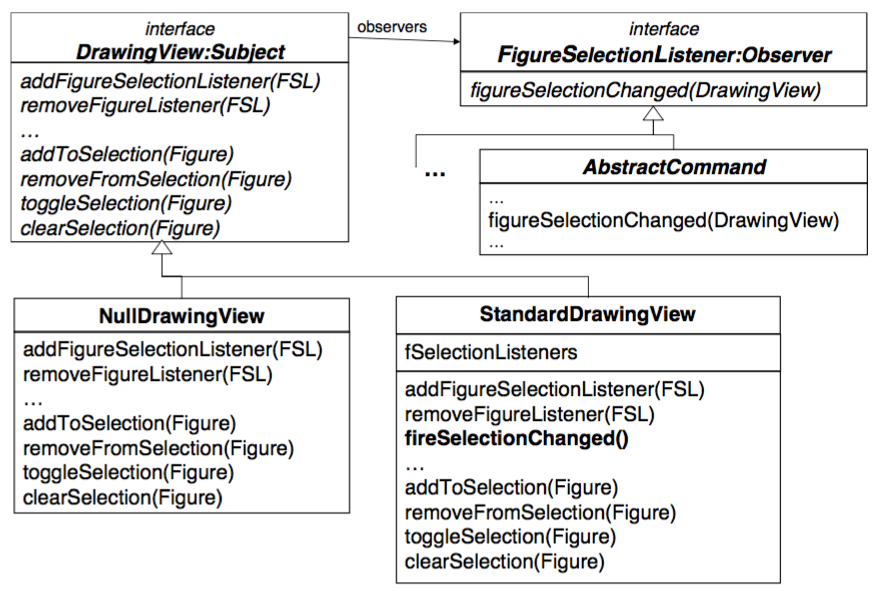
\includegraphics[width=.5\textwidth]{figures/BG_Observer_pattern_Selection_Listener.png}}
  	\caption{Observer pattern: Selection Listener \cite{marin2005approach}}
  	\label{fig:Selection_Listener}
\end{figure}

The \texttt{FigureSelectionListener} interface defines the \textit{Observer} role as its primary concern. 
The interface is implemented by all classes interested in changes of the selection of figures in a drawing view. 
The \texttt{DrawingView} interface partially defines the \textit{Subject} role. 
The \textit{Subject} role is a secondary concern for the \texttt{DrawingView} interface. 
Two classes implement this interface and only one, \texttt{StandardDrawingView}, contains a non-empty implementation of the \textit{Subject} role.

The aspect refactoring would be described as the aspect construct comprises both the \textit{Subject} and \textit{Observer} roles definition and maintains a list of associations between each \textit{Subject} and its \textit{Observer} objects.
The type-based refactoring\cite{marin2005approach} distinguishes several crosscutting elements that occur in an implementation of the \textit{Observer} pattern: role superimposition, applied twice, for each of the two roles and consistent behavior to notify the observers of the changes in the subject object. 
The \texttt{GenericRole} (empty) interface documents the crosscutting type of role superimposition. 
Specific roles, like \textit{Observer} and \textit{Subject} (\texttt{SelectionSubject}) extend the interface.
These elements are shown in the figure \ref{fig:Concerns_Selection_Listener}.

\begin{figure}[H]
	\centering
  	\fbox{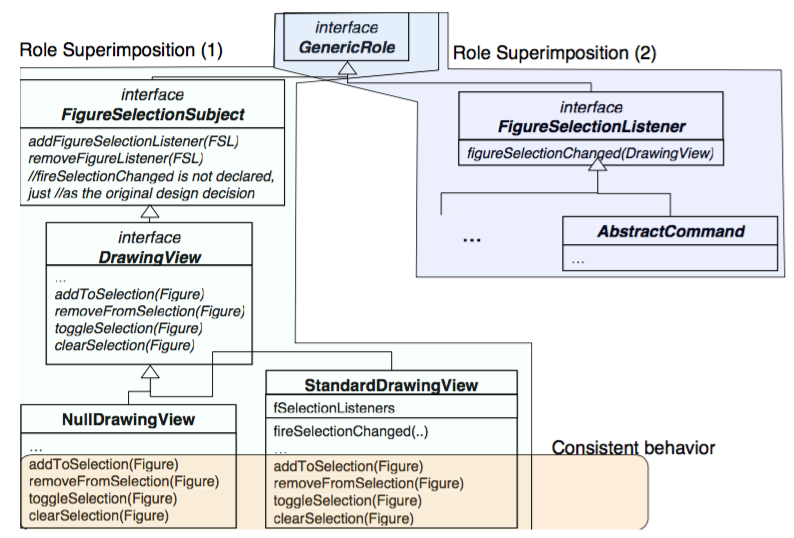
\includegraphics[width=.5\textwidth]{figures/BG_The_concern_types_in_Selection_Listener.png}}
  	\caption{The concern types in Selection Listener \cite{marin2005approach}}
  	\label{fig:Concerns_Selection_Listener}
\end{figure}

%%%%%%%%%%%%%%%%%%%%%%%%%%%%%%%%%%%%%%%%%%%%%%%%%%%%%%%%%%%%%%%%%%%%%%%%%%%%%%%
% \subsubsection{Role-based Refactoring of \acrlong{ccc}}
% \paragraph{Evaluation}
% TODO: Keep it?

%%%%%%%%%%%%%%%%%%%%%%%%%%%%%%%%%%%%%%%%%%%%%%%%%%%%%%%%%%%%%%%%%%%%%%%%%%%%%%%
\subsection{The ``Undo'' Concern of JHotDraw}\label{The Undo Concern of JHotDraw}
After a fan-in analysis of JHotDraw \cite{marin2004identifying}, Marin identified the  ``Undo'' concern in JHotDraw and he presents an approach to the aspect-oriented refactoring of it \cite{marin2004refactoring}. 
He uses the \textit{(un)pluggability} property of a concern as an estimate of its refactoring cost. 
The author proposes the refactoring of the ``Undo'' concern in JHotDraw using AspectJ with the implementation of AJHotDraw. 
During the fan-in analysis \cite{marin2004identifying}, the results have shown about 30 undo activities defined for various elements of JHotDraw. 
A representation of the elements in the JHotDraw implementation of ``Undo'' concern in figure \ref{fig:Participants_for_undo_in_JHotDraw}.

\begin{figure}[H]
	\centering
  	\fbox{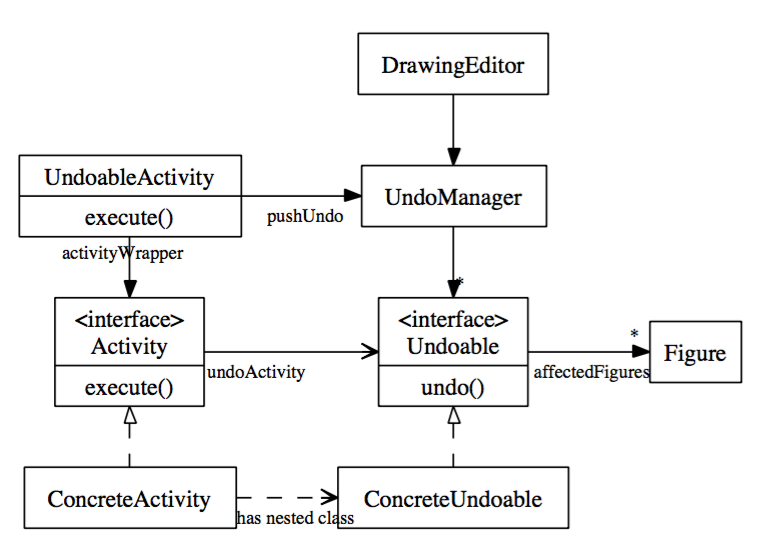
\includegraphics[width=.5\textwidth]{figures/BG_Participants_for_undo_in_JHOTDRAW.png}}
  	\caption{Participants for undo in JHotDraw \cite{marin2004refactoring}}
  	\label{fig:Participants_for_undo_in_JHotDraw}
\end{figure}

The \texttt{Activity} component participates in the implementation of the \textit{Command} design pattern\cite{gamma1995design}. 
Many of these activities have support for undo functionality, which in JHotDraw is implemented by means of nested (undo) classes. 
The nested class knows how to undo the given activity which maintains a list of affected figures whose state is also affected if the activity would be ``undone''. 
Whenever the activity modifies its state it also updates fields in its associated undo activity to actually perform the undo. 
The \texttt{Undoable Command} object serves three roles: 

\begin{itemize}
	\item it consumes the request to execute the command

	\item then, it delegates the command's execution to the wrapped command 

	\item and last, acquires a reference to the undo activity associated with the wrapped command and it pushes it into a stack managed by an \texttt{UndoManager}. 
	When executing an \texttt{Undo Command}, the top undo activity in the stack is extracted and, after the execution of its \texttt{undo()} method, is pushed into a redo stack managed by the same \texttt{UndoManager}.
\end{itemize}

Given this implementation, it is obvious that the primary decomposition of \textit{Command} is crosscut by a number of elements as follows: 

\begin{itemize}
	\item The field by \texttt{AbstractCommand} for storing the reference to the associated \texttt{Undo Activity}.

	\item The accessors for this field implemented by the same class.

	\item The \texttt{UndoActivity} nested classes implemented by most of the concrete commands that support undo.

	\item The factory methods for the undo activities declared by each concrete command that can be undone.
	
	\item The references to the before enumerated elements from non-undo related members.
\end{itemize}

In order to refactor this concern in AspectJ, the implementation of AJHotDraw succeeded though the following steps \cite{marin2004refactoring}:

\begin{enumerate}

	\item An undo-dedicated aspect is associated to each of undo-able command. 
	The aspect will implement the entire undo functionality for the given command, while the undo code is removed from the command class.

 	\item Each aspect will consistently be named by appending \texttt{UndoActivity} to the name of its associated command class to enforce the relation between the two.

	\item Next, the command's nested \texttt{UndoActivity} class moves to the aspect. 
	The factory methods for the undo activities also move to the the aspect, from where are introduced back, into the associated command classes, using inter-type declarations.

	\item Finally, the undo setup is attached to those methods from which was previously removed, namely execute() method, by means of an AspectJ \texttt{advice}.

\end{enumerate}

This proposition \cite{marin2004refactoring} provides an easy migration to an aspect-based solution. 
The \ac{ccc} has been identified, then removed from the system, and finally re-added in an aspect-specific manner.

%%%%%%%%%%%%%%%%%%%%%%%%%%%%%%%%%%%%%%%%%%%%%%%%%%%%%%%%%%%%%%%%%%%%%%%%%%%%%%%
\subsubsection{(Un)pluggability of the Undo concern}
In order to evaluate the \ac{ccc} refactoring of ``Undo'' Marin \cite{marin2004refactoring} used the (Un)pluggability property.

The author groups the commands as complexity assessment based on first the degree of \textit{tangling} of the undo setup in the command's logic, particularly the activity's \texttt{execute()}method and second on the impact of removing the undo-related part from its original site, which can be estimated by the number of references to the factory method and to the methods of the nested undo activity.

Thus, the (un)pluggability property gives a measure of how clear the concern is distinguished in the original code and is a good estimate of the refactoring costs.

%%%%%%%%%%%%%%%%%%%%%%%%%%%%%%%%%%%%%%%%%%%%%%%%%%%%%%%%%%%%%%%%%%%%%%%%%%%%%%%
\subsubsection{AspectJ Drawbacks in the Undo Solution}
By aspect-refactoring now the two concerns are separated, modularized and the secondary concern of undo is no longer tangled into the implementation of the primary one. 
However, a number of drawbacks could overcome by a better aspect language support, which can be discussed in relation to this thesis. 
For instance, since AspectJ's mechanisms do not allow introduction of nested classes, the post-refactoring association will only be an indirect one, based on naming conventions (``\texttt{UndoActivity}''). 
This is a weaker connection than the one provided by the original solution. 
Another drawback that is observed is the change of the visibility of the methods introduced from the aspects, for example the inter-type declarations. 
The visibility declared in the aspect refers to the aspect and not to the target class. 

%%%%%%%%%%%%%%%%%%%%%%%%%%%%%%%%%%%%%%%%%%%%%%%%%%%%%%%%%%%%%%%%%%%%%%%%%%%%%%%
% \subsection{The ``Persistence'' Concern of JHotDraw}


% !TEX root = ../thesis.tex

%%%%%%%%%%%%%%%%%%%%%%%%%%%%%%%%%%%%%%%%%%%%%%%%%%%%%%%%%%%%%%%%%%%%%%%%%%%%%%%
% Chapter: Example Application
%%%%%%%%%%%%%%%%%%%%%%%%%%%%%%%%%%%%%%%%%%%%%%%%%%%%%%%%%%%%%%%%%%%%%%%%%%%%%%%
\chapter{Example Application: State Machine Monitoring}\label{Example Application}
In order to show how our managed data implementation works, in terms aspect refactoring, we to present a showcase in this chapter.
The example consists of a very simple state machines application, which is inspired by Martin Fowler \cite{fowler2010domain}.
The same example is also presented in Enso as a use case for its Object Grammar capabilities \cite{storm2012object}.

Consider the requirements of the state machine are the following: 
\begin{itemize}
	\item A state \texttt{Machine} consists of a number of named \texttt{State} declarations.

	\item Each \texttt{State} contains \texttt{Transitions} to other states, which are identified by a \texttt{name}, when a certain event happens.

	\item A \texttt{Transition} is identified by a certain \texttt{event}.
\end{itemize}

For simplicity, this example will be a very basic \textit{door state machine}, which includes three states \textbf{Open}, \textbf{Close} and \textbf{Locked} accompanied by their transitions: \textbf{open\_door}, \textbf{close\_door}, \textbf{lock\_door} and \textbf{unlock\_door} respectively.
Figure \ref{fig:State_machine} illustrates the door state machine.

\begin{figure}[H]
	\centering
  	\fbox{\includegraphics[width=.50\textwidth]{figures/State_machine.png}}
  	\caption{Basic door state machine}
  	\label{fig:State_machine}
\end{figure}

In order to implement the above we first need to define the models, next interpret the definition given a list of event and finally add any additional functionality (\textit{concern}) needed, for instance monitor the state of the door.

%%%%%%%%%%%%%%%%%%%%%%%%%%%%%%%%%%%%%%%%%%%%%%%%%%%%%%%%%%%%%%%%%%%%%%%%%%%%%%%
\section{Schemas definition}
First, we need to define all the models of the state machine program. 
The object diagram is illustrated in Figure \ref{fig:State_machine_object}.

\begin{figure}[H]
	\centering
  	\fbox{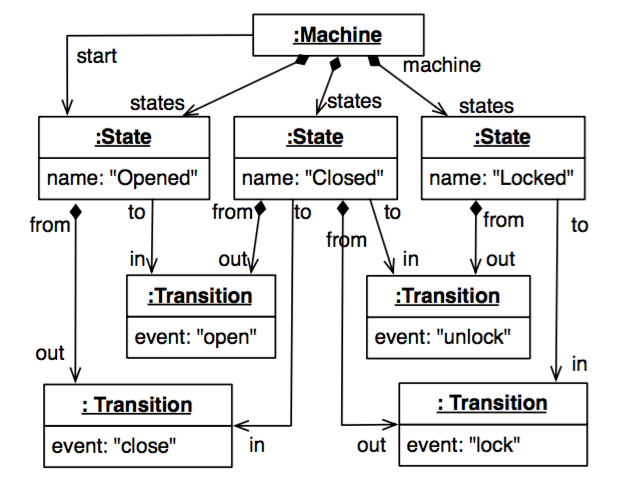
\includegraphics[width=.50\textwidth]{figures/State_machine_object_diagram.png}}
  	\caption{Basic door state machine object diagram}
  	\label{fig:State_machine_object}
\end{figure}

In our implementation we can define schemas using Java interfaces with a set of meta-data described with Java annotation.
Thus, as extracted from the requirements, we need \texttt{Machine} \ref{lst:Machine_Schema}, \texttt{State} \ref{lst:State_Schema}, and \texttt{Transition} \ref{lst:Transition_Schema} models (schemas).

%%%%%%%%%%%%%%%%%%%%%%%%%%%%%%%%%%%%%%%%%%%%%%%%%%%%%%%%%%%%%%%%%%%%%%%%%%%%%%%
\begin{sourcecode}[H]
	\begin{lstlisting}[language=Java,escapechar=|]
public interface Machine extends M {
	State start(State... startingState);

	State current(State... currentState);

	@Contain
	Set<State> states(State... states);
}
	\end{lstlisting}
	\caption{The Machine Schema}
	\label{lst:Machine_Schema}
\end{sourcecode}

As it can be seen in Listing \ref{lst:Machine_Schema}, for the \texttt{Machine} schema definition we need a \texttt{start}ing state, the \texttt{current} state of the machine and a set of \texttt{states} that the machine can be into at each time.
Note that, the \texttt{@Contain} annotation defines that the \texttt{states} field of this schema is part of the spine tree and it is not a cross-reference, but more about it in the implementation Chapter \ref{Schema Definition}.

%%%%%%%%%%%%%%%%%%%%%%%%%%%%%%%%%%%%%%%%%%%%%%%%%%%%%%%%%%%%%%%%%%%%%%%%%%%%%%%
\begin{sourcecode}[H]
	\begin{lstlisting}[language=Java,escapechar=|]
public interface State extends M {
	@Key
	String name(String... name);

	@Inverse(other = Machine.class, field = "states")
	Machine machine(Machine... machine);

	@Contain
	Set<Transition> out(Transition... transition);

	@Contain
	Set<Transition> in(Transition... transition);
}
	\end{lstlisting}
	\caption{The State Schema}
	\label{lst:State_Schema}
\end{sourcecode}

For the \texttt{State} definition, Listing \ref{lst:State_Schema}, we need a \texttt{name} field, which is representing name of the state. 
The \texttt{name} field has been annotated with the \texttt{@Key} annotation, which indicates that state names must be unique and the states field of Machine can be indexed by name.
Moreover, the schema includes a set of \texttt{in} and \texttt{out} \texttt{Transition}s.
Since those two fields are of type \texttt{Set}, that means that a field of the \texttt{Transition} schema has to be marked as key.
In this case is the name (line \ref{line:transition_key} Listing \ref{lst:Transition_Schema}).
Finally, the field \texttt{machine} represents which is the state machine that the current state part of. 
As it can be seen in the schema definition, listing \ref{lst:State_Schema}, the \texttt{machine} field has been annotated with \texttt{@Inverse}, which indicates that this field is a \textit{reference} to a field of an other schema, in this case this schema is the \texttt{Machine} schema and the field is the \texttt{states} field.
Thus, the \texttt{machine} field of \texttt{State} schema is a reference to \texttt{states} field of \texttt{Machine} schema.

%%%%%%%%%%%%%%%%%%%%%%%%%%%%%%%%%%%%%%%%%%%%%%%%%%%%%%%%%%%%%%%%%%%%%%%%%%%%%%%
\begin{sourcecode}[H]
	\begin{lstlisting}[language=Java,escapechar=|]
public interface Transition extends M {
	@Key 					|\label{line:transition_key}| 
	String event(String... event);

	@Inverse(other = State.class, field = "out")
	State from(State... from);

	@Inverse(other = State.class, field = "in")
	State to(State... to);
}
	\end{lstlisting}
	\caption{The Transition Schema}
	\label{lst:Transition_Schema}
\end{sourcecode}

Finally, for the \texttt{Transition} schema definition, Listing \ref{lst:Transition_Schema}, all we need is an \texttt{event} which represents the event of the transition and it is also the \textbf{key}.
Additionally, the \texttt{from} and \texttt{to} states represent the state that the machine changes from and to respectively.
However, those are just reference to the \texttt{State} schema, Listing \ref{lst:State_Schema}, to the \texttt{in} and \texttt{out} fields respectively, since they are defined with the \texttt{@Inverse} annotation.

%%%%%%%%%%%%%%%%%%%%%%%%%%%%%%%%%%%%%%%%%%%%%%%%%%%%%%%%%%%%%%%%%%%%%%%%%%%%%%%
\section{Factory definition}
Since we have our schemas now we need a way to build instances of managed objects of those schemas. 
For Java to create the three schemas as managed data we need to define a factory, which will be the one that creates managed data instances (managed objsects) for each of these schemas \ref{lst:StateMachineFactory}.
Note that those definitions work as \texttt{Constructors} of managed objects.

\begin{sourcecode}[H]
	\begin{lstlisting}[language=Java,escapechar=|]
public interface StateMachineFactory {
	Machine Machine();  // builds a Machine managed object
	State State(); 			// builds a State managed object
	Transition Transition(); // builds a Transition managed object
}
	\end{lstlisting}
	\caption{The StateMachine Factory}
	\label{lst:StateMachineFactory}
\end{sourcecode}

%%%%%%%%%%%%%%%%%%%%%%%%%%%%%%%%%%%%%%%%%%%%%%%%%%%%%%%%%%%%%%%%%%%%%%%%%%%%%%%
\section{Basic Data Manager}
As it is mentioned, in order to interpret and manage the defined data we need data managers. 
Our implementation includes the definition of a \texttt{Basic data manager} that is responsible of making a schema definition to an instance of \textit{managed object}.
However, in order to make the \textit{managed object} it needs its schema definition (the interfaces that define the schemas) and the schema factory (the interface that defines the constructors of the schemas).

%%%%%%%%%%%%%%%%%%%%%%%%%%%%%%%%%%%%%%%%%%%%%%%%%%%%%%%%%%%%%%%%%%%%%%%%%%%%%%%
\subsection{A simple without concerns program}
In the case of a simple program without any concerns, we have to use our managed data to define the state machine and then interpret it.
The definition of the door state machine is given in Listing \ref{lst:Door_state_machine} in Java.

In practice, we need the basic data manager to have a mechanisms that interprets the managed object that comply the \texttt{stateMachineSchema}, shown in Line \ref{line:state_meaning_full_code}.
A a simple interpreter for the state machine is shown in Line \ref{line:state_machine_interpreter}.
As it can be seen, the schemas factory is used to create managed objects and the \textit{wiring} of the fields is done automatically by the data manager who is responsible for the managed object interpretation.

\begin{sourcecode}
	\begin{lstlisting}[language=Java, escapechar=|]
public class StateMachineExample {
	public static void main(String[] args) {
		final Schema schemaSchema = ...; |\label{line:state_schemaSchema}|
		final Schema stateMachineSchema = ....; |\label{line:state_schemaMachineSchema}|

		final BasicDataManager basicDataManagerForStateMachines = 
				new BasicDataManager(StateMachineFactory.class, stateMachineSchema);  |\label{line:state_meaning_full_code}|
		final StateMachineFactory stateMachineFactory = basicDataManagerForStateMachines.make();

		final Machine doorStateMachine = stateMachineFactory.Machine(); |\label{line:state_machine_creation_basic}|

		final State openState = stateMachineFactory.State(OPEN_STATE);
		openState.machine(doorStateMachine);

		final State closedState = stateMachineFactory.State(CLOSED_STATE);
		closedState.machine(doorStateMachine);

		final State lockedState = stateMachineFactory.State(LOCKED_STATE);
		lockedState.machine(doorStateMachine);

		final Transition closeTransition = stateMachineFactory.Transition(CLOSE_TRANSITION);
		closeTransition.from(openState);
		closeTransition.to(closedState);

		final Transition openTransition = stateMachineFactory.Transition(OPEN_TRANSITION);
		openTransition.from(closedState);
		openTransition.to(openState);

		final Transition lockTransition = stateMachineFactory.Transition(LOCK_TRANSITION);
		lockTransition.from(closedState);
		lockTransition.to(lockedState);

		final Transition unlockTransition = stateMachineFactory.Transition(UNLOCK_TRANSITION);
		unlockTransition.from(lockedState);
		unlockTransition.to(closedState);

		doorStateMachine.start(closedState);

		interpretStateMachine(doorStateMachine, new LinkedList<>(Arrays.asList(
		        LOCK_TRANSITION,
		        UNLOCK_TRANSITION,
		        OPEN_TRANSITION)));
	}
}

private static void interpretStateMachine(Machine stateMachine, List<String> commands) { |\label{line:state_machine_interpreter}|
    stateMachine.current(stateMachine.start());
    for (String event : commands) {
        for (Transition trans : stateMachine.current().out()) {
            if (trans.event().equals(event)) {
                stateMachine.current(trans.to());
                break;
            }
        }
    }
}   
	\end{lstlisting}
	\caption{Door state machine}
	\label{lst:Door_state_machine}
\end{sourcecode}

%%%%%%%%%%%%%%%%%%%%%%%%%%%%%%%%%%%%%%%%%%%%%%%%%%%%%%%%%%%%%%%%%%%%%%%%%%%%%%%
\section{Monitoring and notification concerns}
Consider now the case which we want to add some concerns at the previous door state machine implementation.
A simple concern would be a \textit{monitoring} concern, which will log every change in the current state of the state machine.
Another concern would be a \textit{notification} which would be enabled when a specific state is set to the machine.

Suppose, for this example, the system has to notify someone in case the door is opened.
In the case that the door opens, the \textbf{Open} state has set to the current state to the machine, then we want to notify someone by e-mail.
That looks similar to the \textit{monitoring} concern yet, in this case the notification is a specific action; send an e-mail in case the door is open.

\begin{figure}[H]
	\centering
  	\fbox{\includegraphics[width=.50\textwidth]{figures/State_machine_danger.png}}
  	\caption{Simple door state machine: notify closed door}
  	\label{fig:State_machine_danger}
\end{figure}

In order to implement those concerns we need a mechanism that continuously monitors the changes (transitions) of the machine's \texttt{current} state and react accordingly.
In a traditional way this would lead to scattered \textit{monitoring} and \textit{notification} code inside the interpretation method or the models themselves (the machine model).
However, in managed data there are data managers for that purpose.
A data manager can implement concerns as modular aspects without crosscut code to the components.
Therefore, by implementing our concerns with data managers we can keep the interpretation and model definition code, shown in Listing \ref{lst:Door_state_machine}, modular.

%%%%%%%%%%%%%%%%%%%%%%%%%%%%%%%%%%%%%%%%%%%%%%%%%%%%%%%%%%%%%%%%%%%%%%%%%%%%%%%
\subsection{Observable Data Manager}
In order to \textit{observe} for changes in the current state of our door state machine we need a data manager that observes changes in the managed object.
In particular, the \texttt{Machine}'s current \texttt{State}.
This data manager creates concrete managed objects, namely \textit{observable managed object} with which one attach observers that will be notified in case of changes.

%%%%%%%%%%%%%%%%%%%%%%%%%%%%%%%%%%%%%%%%%%%%%%%%%%%%%%%%%%%%%%%%%%%%%%%%%%%%%%%
\subsection{Monitor and notify concerns}
In the example, the observers are the concerns, which are \textit{monitoring} and \textit{notification} by e-mail in case of opened door. 
The definition of those concerns is given in Listing \ref{lst:StateMachineMonitoring}.

\begin{sourcecode} [H]
	\begin{lstlisting}[language=Java, escapechar=|]
public class StateMachineMonitoring {
    public static void monitor(Object obj, String field, Object value) {
        if (field.equals("current")) {
            logger.log(" > Current state changed to " + ((State) value).name());
        }
    }

    public static void notify(Object obj, String field, Object value) {
        if (field.equals("current") && ((State) value).name().equals(OPEN_STATE)) {
            if (EmailSender.send("Danger!", "Someone just opened the door!")) {
            	logger.notify(" > Danger e-mail sent!.");
            }
        }
    }
}
	\end{lstlisting}
	\caption{Door state machine concerns definition}
	\label{lst:StateMachineMonitoring}
\end{sourcecode}

Since there is an observable data manager and the concerns implemented in a separate and reusable module, completely unrelated to our logic code, it is still needed to be integrate them in the door state machine original code.
The integration code is presented in Listing \ref{lst:StateMachineMonitoringConcerns}.
The only part that it changes is the line \ref{line:state_machine_creation_basic} of the original code, in which the data manager of the \texttt{Machine} managed object has changed to the new observable data manager.
Additionally, the concerns are attached to the machine object very easily, as can be seen in lines \ref{line:state_machine_monitor} and \ref{line:state_machine_notify} of Listing \ref{lst:StateMachineMonitoringConcerns}.


\begin{sourcecode} [H]
	\begin{lstlisting}[language=Java, escapechar=|]
...
// State Machine monitoring
final ObservableDataManager observableDataManager = 
			new ObservableDataManager(StateMachineFactory.class, stateMachineSchema);

final StateMachineFactory observableStateMachineFactory = observableDataManager.make();

// Door State Machine definition, with observable data manager
final Machine doorStateMachine = observableStateMachineFactory.Machine();

// Add monitoring and notification concerns
((Observable) doorStateMachine).observe(StateMachineMonitoring::monitor); |\label{line:state_machine_monitor}|
((Observable) doorStateMachine).observe(StateMachineMonitoring::notify);  |\label{line:state_machine_notify}|
...
	\end{lstlisting}
	\caption{Door state machine with concerns}
	\label{lst:StateMachineMonitoringConcerns}
\end{sourcecode}

By running the program with the three commands \texttt{LOCK\_TRANSITION}, \texttt{UNLOCK\_TRANSITION} and \texttt{OPEN\_TRANSITION}, the output is presented in Listing \ref{lst:StateMachineMonitoringConcernsOutput} along with an e-mail sent.
\lstdefinestyle{Bash} {
    backgroundcolor=\color{white},
    basicstyle=\scriptsize\color{black}\ttfamily
}

\begin{sourcecode} [H]
	\lstset{numbers=none}
	\begin{lstlisting}[style=Bash]
> Current state changed to Closed
> Current state changed to Locked
> Current state changed to Open
> Danger e-mail sent!
	\end{lstlisting}
	\caption{Door state machine with concerns: output}
	\label{lst:StateMachineMonitoringConcernsOutput}
\end{sourcecode}

The basic data manager allows to just build managed object, but the observable data manager provided with the functionality of attaching concerns in the managed objects after an specified observed event.
Concluding, that example just presented a modular solution of \ac{ccc} without scattering and tangling code in the components.

% !TEX root = ../thesis.tex

%%%%%%%%%%%%%%%%%%%%%%%%%%%%%%%%%%%%%%%%%%%%%%%%%%%%%%%%%%%
% Chapter: Implementation
%%%%%%%%%%%%%%%%%%%%%%%%%%%%%%%%%%%%%%%%%%%%%%%%%%%%%%%%%%%
\chapter{Managed data in Java}\label{Implementation}

As it has already been mentioned, the programming languages include data definition mechanisms that are predefined. 
This makes them unable to define \ac{ccc} without repeating and scattering code through the components \cite{loh2012managed}.
Notably, the problem is that \ac{ccc} are not considered features of the data types, but instead features of data management.
As a result, we implement managed data to allow the developer to define the mechanisms of data manipulation.
This chapter describes our managed data implementation in Java, testing our first research question, which states \textit{``How to implemented managed data in a static language?''}.
It is important to mention that our implementation is inspired by Enso\footnote{\url{https://github.com/enso-lang/enso}}, which is written in Ruby.
Although Ruby is a dynamic language, Enso significantly contributed to our implementation's design.
In this chapter we preset the implementation of managed data in Java, which is available also online as an open-source project called JavaMD (Java Managed Data)\footnote{\url{https://github.com/TheolZacharopoulos/JavaMD}}.

%%%%%%%%%%%%%%%%%%%%%%%%%%%%%%%%%%%%%%%%%%%%%%%%%%%%%%%%%%%
\section{Managed Data Implementation}\label{sec:Managed Data Implementation}
Managed data allows the programmer to handle the fundamental data manipulation mechanisms using \textit{Data Managers}, one of its distinguishing features being modularity.
Using a data description language the programmer defines \textit{Schemas}. 
\textit{Schemas} are the input of \textit{Data Managers}. 
A \textit{Data Manager} in turn interprets the data description language that is used to define the structure and the behavior of the data to be managed.
\textit{Schemas} and \textit{Data Managers} are essential components of managed data, along with \textit{Integration} in the programming language, in our case being Java.

\subsection{Data description with Schemas}\label{Schema Definition}
To create instances of data, we first need to define their structure.
\textit{Schemas} describe the outline structure of our data.
In order to define \textit{Schemas} in managed data we need a data description language that allows to define records as collections of fields.
This language can be anything, e.g. XML, JSON or a different formalism like the one used in Enso.
For our implementation we chose to use \textbf{Java Interfaces} as a data description language to define records of managed data.
By using Java interfaces we use Java's syntax for our definitions.
Moreover, Java interfaces use several conventions to encode semantics, for instance Java annotations, which are very useful for meta data definition on \textit{Schema}s.

As a result, to define a \textit{Schema} we first need to define a set of classes that describe that schema.
A schema \texttt{Klass} \footnote{
	We use the ``Klass'' instead of ``Class'' convention in order to avoid any kind of ambiguities between Java's Class type and our type system. Klass is used to describe our own class type while Class describes Java's native class type.} 
is described by a name and a set of \texttt{Field}s, each of which has a name and a \texttt{Type}.
Since Java interfaces are used to define a \texttt{schemaKlass} we need a way to define \texttt{Field}s for that \texttt{schemaKlass}.
A \texttt{Field} in our data description language can be defined by using \textbf{Java's Method} definition.

Additionally, there are several attributes, considered meta data, that help define the structure of a \texttt{Schema}.
In order to define the meta data in our data description language (interfaces), we use \textit{Java Annotations}.
Annotations are very declarative in the way they express meta data in interfaces and they are consistent with the system (Java).

Thus, to provide a field with meta data, we define annotations in a \textit{Method} target level since a \texttt{Field} is defined by a \textit{Method} declaration Java interfaces.

Note that by using Java interfaces and annotations for our schemas definition, we gain a first level of type checking from \ac{jvm}. 
The reason is that before we run our runtime interpretation of schemas, \ac{jvm} performs type checking in the definitions and in case of wrong types it notifies the programmer.
Additionally, this is beneficial when a programmer uses IDE's that perform real time type inspection\footnote{\url{https://www.jetbrains.com/help/idea/15.0/code-analysis.html}}. 
In those cases errors on the definitions will be spotted immediately. 

The list of the available structure concepts that are supported in our language is presented below \cite{loh2012managed}:
\begin{description}
	\item [@Key] When a method (field definition) is annotated with the \texttt{@Key} annotation that forces its value to be unique within collections of this field's Klass.
	The key should be used on a single field of a Type and its value represents the uniqueness of its Klass's instance.
	Another way to look at this is as a counterpart of the \texttt{hashCode} in traditional Java programs.
	This way when many values of a Klass are in a Set, the key field ensures uniqueness in its context.

	\item [@Inverse] This annotation includes two \textit{annotation element definitions} \footnote{
		\url{https://docs.oracle.com/javase/tutorial/java/annotations/declaring.html}}.
	When a method is annotated with the \texttt{@Inverse(Class other, String field)} annotation, then the inverse \texttt{field} element must be a \texttt{Field}'s name in the \texttt{Class} interface, given by the \texttt{type} element.
	This meta data is used as a reference declaration in schemas, meaning that when a programmer updates the value of a field that is annotated with inverse, then the value of the field that refers to will be also updated.
	This mechanism is interpreted by the managed object and is used for automated \textit{wiring} of the field across a schema.

	\item [@Contain] When a field is annotated with the \texttt{@Contain} annotation, then this field is considered as \textit{traversal}. 
	In general, traversals describe a minimum spanning tree that is called \textit{spine} and ensures reachability of values.
	The spine is used in implementations that need a depth-first search by distinguishing between the actual information and the cross-references of the spanning tree.
	If a spanning tree is defined, then all nodes in a model must be uniquely reachable by following just the spine fields \cite{storm2012object}.
	An example of such functionality is the equivalence between managed objects that is presented in Section \ref{Managed Object equivalence}.
	Sometimes traversal fields describe composition, or ``is a part of'', relationships \cite{loh2012managed}.

	\item [@Optional] When the \texttt{@Optional} annotation is on a field's definition this field can include \texttt{null} values.
	\texttt{Inverse} fields are \texttt{Optional}. 

	\item [Java Inheritance] In addition to the Java annotations, our language uses more Java mechanisms for schemas definition. 
	Java inheritance is one of them. 
	A \texttt{schemaKlass} can extend another Klass (super), which works as the traditional Java inheritance, supporting sub typing mechanisms.
	Implementing this we introduce a \textit{Type Hierarchy} model that includes super and sub classes on managed objects.
	Note that since we use interfaces for \texttt{schemaKlass}, we implicitly support multiple inheritance because a Java interface can extend more than one interfaces.

	\item [Java Collections] Finally, another Java mechanism that we use is the definition of a field that includes many values.
	To define such a field, a programmer has to declare a field's \texttt{Type} as a \texttt{java.util.List} or a \texttt{java.util.Set} of this \texttt{Type}.

\end{description}

Using all the aforementioned constructs of our data definition language, a programmer can define any kind of schema, even itself (see Section \ref{Self-Describing Schemas}).
Schema definition examples are presented in Chapter \ref{Example Application} Listings \ref{lst:Machine_Schema}, \ref{lst:State_Schema} and \ref{lst:Transition_Schema}.
In those definitions the above concepts can be recognized and their meaning can be revealed in context.

%%%%%%%%%%%%%%%%%%%%%%%%%%%%%%%%%%%%%%%%%%%%%%%%%%%%%%%%%%%
\subsection{IFactories}\label{IFactories}
However, even if we have the definitions of schemas, we still need a way to create instances of managed data described by them.
We can not use Java's mechanisms\footnote{\texttt{new} keyword} for this functionality since we need them to be managed data and not ordinary objects.
Thus, we use Java interfaces to define instance factories.
An \texttt{IFactory} interface extension is a list of \textit{constructor definitions} for specific schemas.
% #Important
The \texttt{IFactory} interface is an empty interface that is used for documentation and semantics manner.

The methods in the interfaces that extend \texttt{IFactory} are used similarly to the constructors in a Java class, while their implementation is handled by the data managers.
Since those methods are constructors, we can define a constructor with or without initial values.
Unfortunately, we have encountered a limitation regarding constructors with initialization values, making them inappropriate to use in complicated schemas.

%%%%%%%%%%%%%%%%%%%%%%%%%%%%%%%%%%%%%%%%%%%%%%%%%%%%%%%%%%%
\subsubsection{Methods Ordering Issue}\label{Methods ordering}
The problem lays on Java's reflection mechanisms in terms of methods ordering.
More specifically, when the methods of a \texttt{java.lang.Class} are requested by using the \texttt{public Method[] getMethods()} method\footnote{
	As it is mentioned in \url{https://docs.oracle.com/javase/8/docs/api/java/lang/Class.html\#getMethods--}, the elements in the returned array are not sorted and are not in any particular order.}, 
the returned values are not ordered the way as defined in the source code.
Consequently, since the schema definition is reflectively analyzed in the data managers and is dependent on that order, those methods can not be used in the initialization of values.

However, we overcame this difficulty and were able to support this feature in an alternative manner.
In our implementation both the defined methods and the fields are \textbf{alphabetically ordered} by name before being initialized.

That feature can be used by the programmer although it can be confusing.
Therefore, as an advice, we suggest to either provide constructors without initialization values or to write constructors with only \textbf{primitive} initialization values in \textbf{alphabetical order}.
Otherwise we risk getting values in a random order leading to an error or a wrong value assignment.

%%%%%%%%%%%%%%%%%%%%%%%%%%%%%%%%%%%%%%%%%%%%%%%%%%%%%%%%%%%
\subsection{Data Managers Implementation}\label{Data Managers Implementation}
However, the schemas are not a complete managed data specification without a corresponding \texttt{Data Manager}.
A data manager is responsible for interpreting the schema and building virtual objects (managed objects). 
The managed object's fields are defined by the given schema and acts according to the specifications given by the data manager.
Additionally, the data manager ensures that the data given are valid with respect to the schema.
More specifically, the data managers describe how a schema definition is handled from the outside world and what its specifications are.
These properties may include \ac{ccc} that can be described separately by special data managers, separating schema and concern definitions.
Thus, a managed object can have multiple interpretations based on the data manager that is used to interpret it.

A data manager is initialized with a \texttt{Schema} and provides a new \texttt{Managed Object} instance whose properties are defined by that data manager.
Additional to the \texttt{Schema} that includes a Set of \texttt{Type}s (\texttt{Primitive}s or \texttt{Klass}es), it also needs a \texttt{IFactory} that declares the constructors of the given schema \texttt{Klass}.
The data manager through its \texttt{factory} method interprets the schemas and builds new \texttt{IFactories}, which in turn create \texttt{Managed Objects} with the specifications of the data manager.

In the example presented in listing \ref{lst:Basic data Manager Example}, Line \ref{line:basic_data_manager_definition} defines a basic data manager.
This data manager gets the \texttt{IFactory} and the \texttt{Schema} of a state machine as input in the \texttt{factory} method. 
Next, Line \ref{line:basic_data_manager_schema_factory_definition} shows a new \texttt{IFactory} instance is being created, which builds managed objects with the specifications attached from the basic data manager.
Finally, Line \ref{line:basic_data_manager_definition_instance} illustrates how the managed object instances with those specifications can be built.

\begin{sourcecode} [H]
	\begin{lstlisting}[language=Java, escapechar=|]
// Create a basic data manager for state machines
BasicDataManager basicDataManagerForStateMachines = new BasicDataManager(); |\label{line:basic_data_manager_definition}|

// Create a factory that makes managed objects 
// with the specifications of the basic data manager.
StateMachineFactory stateMachineFactory = basicDataManagerForStateMachines
		.factory(StateMachineFactory.class, stateMachineSchema); |\label{line:basic_data_manager_schema_factory_definition}|

// Build an instance of managed object with those specifications.
Machine stateMachineInstance = stateMachineFactory.Machine(); |\label{line:basic_data_manager_definition_instance}|
	\end{lstlisting}
	\caption{Basic data Manager Example}
	\label{lst:Basic data Manager Example}
\end{sourcecode}

\subsubsection{Basic Data Manager}
As described above, we use Java interfaces to define schema Klasses that include fields. 
Those fields are dynamically discovered by a schema loading process and provided to the data manager as schemas.
A data manager has the ability to determine the fields and methods of the managed object during runtime.
In addition, when the data manager adds functionality on a managed object then it first delegates the calls to its specifications and then to the fields of an instance.
In order to dynamically interpret a schema inside a data manager and delegate its functionalities, we used Dynamic Proxies.

In our implementation we have separated the Proxy factory (\texttt{DataManager}) from the Invocation Handler (\texttt{MObject}).
This way, the \texttt{DataManager} class is responsible for creating proxy instances of \texttt{IFactories}. 
The \texttt{IFactory} creates proxy instances with the \texttt{MObject} class instances as invocation handlers.
The \texttt{MObject} instances are responsible for interpreting the schema and delegating actions using their invocation handling implementation. 
Figure \ref{fig:DataManager_and_MObject} illustrates this structure.
As it can be seen the data manager is a \textit{factory} that has a single exposed method, \texttt{factory()}, that is used to build an \texttt{IFactory} instance, which in turn builds \texttt{MObject} instances.

\begin{figure}[H]
	\centering
  	\fbox{\includegraphics[width=.85\textwidth]{figures/DataManager_and_MObject.png}}
  	\caption{Data Manager and MObject}
  	\label{fig:DataManager_and_MObject}
\end{figure}

The two level \textit{proxing} process that the \texttt{DataManager} class performs, from the basic data manager to IFactory and then to MObject, can be seen in Listing \ref{lst:Basic Data Manager}.
Note that the \texttt{createManagedObject} is \texttt{protected} for the sub data managers to override it in order to create MObjects of preference.
In addition the \texttt{createManagedObjectProxy} is also \texttt{protected} in case the programmers wants to to extend the proxy creation.

\begin{sourcecode} [H]
	\begin{lstlisting}[language=Java, escapechar=|]
public <T extends IFactory> T factory(
	Class<T> factoryClass, Schema schema, Class<?>... additionalInterfaces) 
{
	// add the extra proxy interfaces
	for (Class<?> proxyInterface : additionalInterfaces) {
		this.addProxyInterface(proxyInterface);
	}

	// add the klass interfaces of the schema
	for (Klass klass : schema.klasses()) {
		this.addProxyInterface(klass.classOf());
	}

	return (T) Proxy.newProxyInstance(
		factoryClass.getClassLoader(),
		new Class<?>[]{factoryClass},
		(proxy, method, args) -> // invocation handler
			createManagedObjectProxy(factoryClass, schema, method, args) // mobject
		);
}

protected Object createManagedObjectProxy(...) {
	//...
	MObject managedObject = createManagedObject(schemaKlass, inits); // invoc handler
	return Proxy.newProxyInstance(
		schemaFactoryCallingMethodClassLoader, // schema constructor
		proxiedInterfaces.toArray(new Class[additionalInterfaces.size()]),
		managedObject
	);
}
\end{lstlisting}
	\caption{Basic Data Manager}
	\label{lst:Basic Data Manager}
\end{sourcecode}

\subsubsection{Stacking Data Managers}
In order to create a stack of data managers that combine behavior and specifications, we can use inheritance.
Figure \ref{fig:DataManager_and_MObject} shows how this works.
In detail, \texttt{AnotherDataManager} extends \texttt{BasicDataManager} and simply overrides the \texttt{createManagedObject} and the \texttt{factory} methods.
The \texttt{createManagedObject} method is responsible for creating a new instance of an \texttt{MObject}.
In this case, the \texttt{createManagedObject()} method will create a new \texttt{AnotherMObject} instance.
The \texttt{factory} method is responsible of creating a new \texttt{IFactory} instance.
Note that it is important that the data managers inherit from a base data manager, leading to the modular aspect of the data managers.
As it can be seen, for stacking data managers we used the \textit{Decorator Pattern} \cite{gamma1995design} which is mentioned also in Cook et al. \cite{loh2012managed} as a strategy for static \ac{oop} languages.

%%%%%%%%%%%%%%%%%%%%%%%%%%%%%%%%%%%%%%%%%%%%%%%%%%%%%%%%%%%
\subsection{MObjects}\label{sec:Managed Objects}
The \texttt{MObject}, is an implementation of the \texttt{InvocationHandler} interface.
Thus, the \texttt{MObject}'s \texttt{invoke()} method is called in every field access of the managed object's instance.
To manipulate its fields' values this object has two methods, \texttt{\_set()} and \texttt{\_get()}.
In the implementation of these methods additional checks are performed to ensure the correctness of types and structure of the values.
Therefore, a type checker in the schemaKlass level has been implemented in the particular place.
The setter and getter methods can be overridden from derived \texttt{MObject}s in order to \textit{Decorate} the basic \texttt{MObject} with their functionality. 
Of course they require to call their \texttt{supers} for running the type checker.

The \texttt{MObject} is the \textit{backing object} that stores a reference to the \texttt{schemaKlass} and its implementation represents an instance of that \texttt{schemaKlass}.
That \texttt{schemaKlass} is a meta class that describes the layout of the \texttt{MObject} and keeps the \texttt{Field}s and their \texttt{Types}.
During construction, the fields of the \texttt{MObject} are specified by its \texttt{schemaKlass}.
When a field check has to be performed, the \texttt{MObject} uses its \texttt{schemaKlass}.

Overall, one can easily argue that this class defines the main functionality of managed data.
In particular, this class is the \textit{interpreter} of managed data.
Therefore, it is responsible for handling the calls to methods (invocation handler), invoke default methods, setup and initialize field values, based on its \texttt{schemaKlass}, and internally perform the \textit{type checking}.
A detailed presentation of this class and its action is explanation in Appendix \ref{apdx:MObject}.

%%%%%%%%%%%%%%%%%%%%%%%%%%%%%%%%%%%%%%%%%%%%%%%%%%%%%%%%%%%%
%%%%%%%%%%%%%%%%%%%%%%%%%%%%%%%%%%%%%%%%%%%%%%%%%%%%%%%%%%%%
\subsection{Implementing a Data Manager}\label{Implementing a Data Manager}
The implementation and the integration of a new data manager is straight forward in our framework.
As it can be seen in Figure \ref{fig:DataManager_and_MObject}, the basic components of a new data manager implementation are the \texttt{Data Manager} class (proxy) and the \texttt{MObject} class (invocation handler).

First, to follow the modularity aspect and the ability to stack data managers together combining their specifications, we need to inherit from, at least, the \texttt{BasicDataManager} and its \texttt{MObject} respectively.
A simple data manager that could be useful is a data manager that introduces immutability to its managed objects.
A \texttt{Lockable} data manager should first inherit the \texttt{BasicDataManager} to get its field access specification.
The implementation of the \texttt{LockableDataManager} is illustrated in \ref{lst:Lockable Data Manager}.

\begin{sourcecode} [H]
	\begin{lstlisting}[language=Java, escapechar=|]
public class LockableDataManager extends BasicDataManager {

	@Override
    public <T extends IFactory> T factory(
    	Class<T> factoryClass, Schema schema, Class<?>... additionalInterfaces) {
        // Add the Lockable class in order to use it in the managed object.
        return super.factory(factoryClass, schema, Lockable.class);
    }

	@Override
	protected MObject createManagedObject(Klass klass, Object... _inits) {
		return new LockableMObject(klass, _inits);
	}
}
	\end{lstlisting}
	\caption{Lockable Data Manager}
	\label{lst:Lockable Data Manager}
\end{sourcecode}

Additionally, it should add some \textit{locking} mechanism to ensure immutability of its objects.
This is defined in the \texttt{Lockable} interface, which is responsible of ensuring the implementation of the specifications. 
Listing \ref{lst:Lockable Interface} shows the specifications of the interface.

\begin{sourcecode} [H]
	\begin{lstlisting}[language=Java, escapechar=|]
public interface Lockable {
	void lock();
}
	\end{lstlisting}
	\caption{Lockable Interface}
	\label{lst:Lockable Interface}
\end{sourcecode}

Since we have the specifications and the data manager that creates the \textit{Lockable} managed object, we still need the implementation.
The implementation is located in the \texttt{MObject} and in this case the \texttt{LockableMObject}, 
Listing \ref{lst:Lockable Managed Object}.

\begin{sourcecode} [H]
	\begin{lstlisting}[language=Java, escapechar=|]
public class LockableMObject extends MObject implements Lockable {
	private boolean isLocked = false;

	public LockableMObject(Klass schemaKlass, Object... initializers) {
		super(schemaKlass, initializers);
	}

	public void lock() {
		isLocked = true;
	}

	@Override
	public void _set(String name, Object value) 
	throws NoSuchFieldError, InvalidFieldValueException, NoKeyFieldException {
		if (isLocked)
	    	throw new IllegalAccessError(
	    		"Cannot change " + name + " of locked object " + schemaKlass.name() + ".");
		super._set(name, value);
	}
}
	\end{lstlisting}
	\caption{Lockable Managed Object}
	\label{lst:Lockable Managed Object}
\end{sourcecode}

The \texttt{LockableMObject}, by extending the \texttt{MObject} and implementing the \texttt{Lockable} interface, inherits the basic functionality of a managed object and gets a specification description respectively.
Its role is to implement the logic of the immutability, which is as simple as it looks.
In order to use this functionality, one needs to create managed objects using this data manager.
An example is shown in Listing \ref{lst:Immutability Example}.

\begin{sourcecode} [H]
	\begin{lstlisting}[language=Java, escapechar=|]
LockableDataManager lockableFactory = new LockableDataManager();
PointFactory lockablePointFactory = 
	lockableFactory.factory(PointFactory.class, pointSchema);
Point2D lockablePoint = lockablePointFactory.Point2D(1, 2);

// It was mutable until now, now it is locked (immutable).
((Lockable)lockablePoint).lock();
try {
	lockablePoint.x(2); // Should throw here since its immutable.
} catch (IllegalAccessError e) {
	System.err.println("IllegalAccessError: " + e.getMessage());
}
	\end{lstlisting}
	\caption{Immutability Example}
	\label{lst:Immutability Example}
\end{sourcecode}

%%%%%%%%%%%%%%%%%%%%%%%%%%%%%%%%%%%%%%%%%%%%%%%%%%%%%%%%%%%
\section{Self-Describing Schemas}\label{Self-Describing Schemas}
As explained by Cook et al. \cite{loh2012managed}, a self-describing schema is a schema that can be used to define schemas, including itself.
Our framework is fully self-described, the schemas are also described by schemas which are both models \cite{kurtev2006model}. 
To allow schemas to be managed data we need a ``self-describing schema mechanism'' or \textit{SchemaSchema}.
Through the \textit{SchemaSchema} the approach of managed data can be applied at the meta level as well.

The reason that a self-describing schema is important is because schema schemas can be used from factories (IFactory) to create schemas.
The schema of schemas is just a schema that allows the creation of schemas, including its own schema \cite{storm2012object}.
Additionally, by presenting the schema as the first-class model\cite{kurtev2006model}, they can be extended in the same way just like ordinary models.

\subsection{SchemaSchema}\label{sec:SchemaSchema}
By using Java interfaces the \textit{Schema} classes are tightly coupled structurally to the Java interfaces used to define them.
Since we want to decouple from Java interfaces and reflection we need our own \textit{Klass system}.
In order to be self-describing we want this Klass system to be also represented as managed data. 
To model the structure of a \texttt{Schema} itself we need to be able to describe a class as a collection of \texttt{Fields}, each of which has a \texttt{name} and a \texttt{Type} \cite{loh2012managed}. 
Thus, for our \textit{SchemaSchema} definition we need a \texttt{Type}, a \texttt{Field} and a \texttt{Schema} as a collection of \texttt{Type}s. 
A \texttt{Type} could be both a \texttt{Primitive}, without \texttt{Fields}, and a \texttt{Klass}, with a set of \texttt{Fields}.
Additionally, those \texttt{Fields} may have some extra meta data attributes that are explained in Section \ref{Schema Definition}.

A schema like this can describe itself since every concept used in the explanation is de facto included in the definition.
For a self-describing implementation we need to describe our own SchemaSchema. 

Figure \ref{fig:SchemaSchema_definition} illustrates the modeling of this definition.

\begin{figure}[H]
	\centering
  	\fbox{\includegraphics[width=.85\textwidth]{figures/SchemaSchema_definition.png}}
  	\caption{The schema of schemas}
  	\label{fig:SchemaSchema_definition}
\end{figure}

\subsection{SchemaFactory}\label{sec:SchemaFactory}
Considering that we have the schema of our schema (\textit{SchemaSchema}) we need a way to create instances of those \textit{schemaSchemaKlasses}.
In this case, as we do with the normal schemas, we use an IFactory definition.
However, this time it is a \textit{SchemaFactory} that defines constructors of all the schema klasses that are needed to describe our \textit{SchemaSchema}.
Listing \ref{lst:SchemaFactory} shows its definition.

\begin{sourcecode} [H]
	\begin{lstlisting}[language=Java, escapechar=|]
public interface SchemaFactory extends IFactory {
    Schema Schema();
    Primitive Primitive();
    Klass Klass();
    Field Field();
    Field Field(
    	Boolean contain, Boolean key, Boolean many, String name, Boolean optional);
}
	\end{lstlisting}
	\caption{SchemaFactory}
	\label{lst:SchemaFactory}
\end{sourcecode}

%%%%%%%%%%%%%%%%%%%%%%%%%%%%%%%%%%%%%%%%%%%%%%%%%%%%%%%%%%%
\subsection{Schema Loading}\label{sec:Schema Loading}
To construct the Klass system we need to analyze the Java interfaces using reflection and then build actual instances of the Schema, Klass, Field etc. using the appropriate factory.
The \texttt{SchemaLoader} is responsible of this process.

\texttt{SchemaLoader}'s \texttt{load} static method takes as input a Set of interfaces, which are the schema definitions, a \texttt{SchemaFactory} that includes constructor definitions of the \texttt{SchemaSchema} and returns a new instance of \texttt{Schema}.
During the reflective analysis of the input interfaces the \texttt{SchemaLoader} builds the corresponding \texttt{Types} and \texttt{Fields} of those interfaces using the \texttt{SchemaFactory}.
A \texttt{Schema} consists of the Set of these \texttt{Types}.
An example taken from Chapter \ref{Example Application}, is shown in Listing \ref{lst:SchemaLoader Example}.

\begin{sourcecode} [H]
	\begin{lstlisting}[language=Java, escapechar=|]
Schema schemaSchema = ...;
SchemaFactory sf = basicFactory.factory(SchemaFactory.class, schemaSchema);

Schema stateMachineSchema = SchemaLoader.load(
	sf, Machine.class, State.class, Transition.class);
	\end{lstlisting}
	\caption{SchemaLoader Example}
	\label{lst:SchemaLoader Example}
\end{sourcecode}

In its implementation, the \texttt{SchemaLoader} gets as input a \texttt{SchemaFactory} and a set of interfaces that describe the state machine schema.
Next, it returns a new instance of the state machine Schema.
This schema consists of a set of schema Klasses that are described by interfaces, namely \texttt{Machine.class}, \texttt{State.class} and \texttt{Transition.class}.
Next, the \texttt{SchemaLoader} analyzes the definition of those schemas using reflection and then makes a \texttt{Schema} by using the \texttt{SchemaFactory} that it has been given.
A more detailed description of this process is given in Appendix \ref{appdx:SchemaLoading}.
% #important
In general \texttt{SchemaLoader} can be seen as our parser, which accepts a description of language (the interfaces) and a method create objects of its components (the schema factory).

%%%%%%%%%%%%%%%%%%%%%%%%%%%%%%%%%%%%%%%%%%%%%%%%%%%%%%%%%%%
\section{Bootstrapping}\label{sec:Bootstrapping}
Considering that SchemaSchema is managed data itself, we can use the SchemaLoader to build a new SchemaSchema.
Nonetheless, we need a description of that SchemaSchema, which will be used during the loading process to build the schema Klasses.
As a result, we need a \textit{Bootstrap Schema} to jumpstart this process.
The \textit{Bootstrap Schema} is exclusively self-describing, as it must manage itself \cite{loh2012managed}, and hardcoded in its own class, \texttt{BootSchema}.

\subsection{Cutting the umbilical cord}\label{subsec:Cutting the umbilical cord}
Having a \texttt{BootSchema} in place we can now create ``real'' \texttt{SchemaSchema}s \footnote{
	We call them real because they are managed data and not hard-coded.}.
For consistency, we use those ``real'' \texttt{SchemaSchema}s in order to build other schemas, this way everything is managed data.
After building a real SchemaSchema we no longer need the \texttt{BootSchema}, which leads to a process that we call ``Cutting the umbilical cord''.
An example of ``Cutting the umbilical cord'' is shown in Listing \ref{subsec:Cutting the umbilical cord}, where we use the \texttt{BootSchema} to build the \texttt{realSchemaSchema} and then we use this \texttt{realSchemaSchema} to build another \texttt{realSchemaSchema} (\texttt{realSchemaSchema2}).

\begin{sourcecode} [H]
	\begin{lstlisting}[language=Java, escapechar=|]
final BasicDataManager basicFactory = new BasicDataManager();
final SchemaFactory schemaFactory = 
	basicFactory.factory(SchemaFactory.class, new BootSchema());
final Schema realSchemaSchema = SchemaLoader.load(
        	schemaFactory,
         	Schema.class, Type.class, Primitive.class, Klass.class, Field.class,
        	Primitives.class); |\label{line:Primitives}|

final BasicDataManager basicFactory2 = new BasicDataManager();
final SchemaFactory schemaFactory2 = 
	basicFactory2.factory(SchemaFactory.class, realSchemaSchema);
final Schema realSchemaSchema2 = SchemaLoader.load(
        	schemaFactory2, 
        	Schema.class, Type.class,  Primitive.class, Klass.class, Field.class);
	\end{lstlisting}
	\caption{Cutting the umbilical cord}
	\label{lst:Cutting the umbilical cord}
\end{sourcecode}

Figure \ref{fig:schema_schema_models} illustrates the models during a bootstrapping process.
As it can be seen, the \texttt{BootSchema} is used in order to describe the Schema Schema, making the Schema Schema independent and managed data itself.
Thus, it can be used to create other schemas like the Machine schema or even itself.

\begin{figure}[H]
	\centering
  	\fbox{\includegraphics[width=.4\textwidth]{figures/schema_schema_models.png}}
  	\caption{Boot Schema models}
  	\label{fig:schema_schema_models}
\end{figure}

\subsection{Primitives Definition}\label{Primitives Definition}
Since the Bootstrap Schema defines the primitive types for its description, the real schema schema needs a way to include them as well.
These initial Java primitives supported in our implementation are shown in Table \ref{tbl:primivites_table}.

\begin{table}[H]
	\centering
	\begin{tabular}{@{}lccc@{}}
	\toprule
	                 & \textbf{Class} & \textbf{Name} & \textbf{Default Value} \\ \midrule
	\textbf{Integer} & Integer.class  & ``Integer''   & 0                      \\
	\textbf{int}     & int.class      & ``int''       & 0                      \\
	\textbf{Boolean} & Boolean.class  & ``Boolean''   & false                  \\
	\textbf{boolean} & boolean.class  & ``boolean''   & false                  \\
	\textbf{String}  & String.class   & ``String''    & ``''                   \\
	\textbf{Double}  & Double.class   & ``Double''    & 0.                     \\
	\textbf{Float}   & Float.class    & ``Float''     & 0.f                    \\
	\textbf{Class}   & Class.class    & ``Class''     & null                   \\
	\textbf{Object}  & Object.class   & ``Object''    & null                   \\ \bottomrule
	\end{tabular}
	\caption{Primitives Table}
	\label{tbl:primivites_table}
\end{table}

To define those primitives we use an interface called \textit{Primitives}, introduced during the loading of the real schema, as seen in Line \ref{line:Primitives} of Listing \ref{lst:Cutting the umbilical cord}.
The definition of this interface is shown in Listing \ref{Primitives Definition} which is a simple \texttt{Class/Name} mapping \footnote{We use the ``\_'' prefix convention in order to define names of primitives that are reserved words in Java.}. 

\begin{sourcecode} [H]
	\begin{lstlisting}[language=Java, escapechar=|]
public interface Primitives {
	Integer Integer();
	int _int();
	Boolean Boolean();
	boolean _boolean();
	String String();
	Class Class();
	Float Float();
	Double Double();
}
	\end{lstlisting}
	\caption{Primitives Definition}
	\label{lst:Primitives Definition}
\end{sourcecode}

The benefits of such a definition is that the \texttt{Primitives} interface is extensible.
By extending it one can add more primitives in the schema as long as it is introduced during the schema loading.

%%%%%%%%%%%%%%%%%%%%%%%%%%%%%%%%%%%%%%%%%%%%%%%%%%%%%%%%%%%%
\section{Implementation Issues}\label{Implementation Issues}
The fact that we use Java reflection and dynamic proxies, along with the fact that everything is managed data, even the schemaSchema, introduces some issues, including the methods ordering problem described in Section \ref{Methods ordering}.

\subsection{Equivalence}\label{Managed Object equivalence}
The \texttt{bootstrapSchema}, \texttt{realSchemaSchema} and \texttt{realSchemaSchema2} managed objects from the Listing \ref{subsec:Cutting the umbilical cord} should be equal because they ultimately describe the same \textit{Schema}.

However, since, apart from the \texttt{bootstrapSchema}, they are managed data and not normal Java objects, we need a way to check for equality on managed objects.
We have implemented the equivalence functionality for managed objects, using the \textit{Equality Checking for Trees and Graphs
algorithm} by Michael D. Adams and R. Kent Dybvig \cite{adams2008efficient}.

\subsection{The classOf field}\label{The classOf field}
As it has be presented in Section \ref{Dynamic Proxies}, for a proxy object to conform with interfaces and be casted to any of them, it needs these interfaces during its initialization.
To support that, we have added the \texttt{classOf} field in the \texttt{Type} schema Klass, which is of type \texttt{java.lang.Class} and is a reference of the Java class that this schema Klass is described to.

\subsection{Hash-code of Managed Objects}\label{Hashcode of Managed Objects}
To avoid any unpredictable activities that a \texttt{hashCode} invocation would bring in managed objects, we have omitted it. 
We do not depend on the ordinary \texttt{hashCode} for managed objects, we do not call it and therefore we have not implemented it.
If it is a collection field type, then the field has to have a \texttt{Key} field. 
In this case, we obtain the value of the key field and index it into a \texttt{HashMap}. 

Using the \texttt{Key} field as the key of the hashmap works whether it is a primitive or not since we get the \texttt{Object.hashCode()} of that key.
However, that suggests that the key is not of our schema Klass system but a Java type.
Finally, the \texttt{MObject} invocation handler delegates the call of the \texttt{hashCode} method to the real object so that it would never fail, although this is not suggested because it may lead to unpredictable results.

\subsection{Java 8 Default Methods}\label{Java 8 Default Methods}
Java 8 supports the definition of default methods in interfaces.
According to the specification\footnote{\url{https://docs.oracle.com/javase/tutorial/java/IandI/defaultmethods.html}}, default methods enable the programmer to add new functionalities to the interfaces and can be used as method implementation in abstract classes.
We use Java 8 default methods in order to add functionality to our schema definitions. 
In particular, methods that are defined as \textit{default} are ignored during the interpretation and no fields are created for them.
We consider this as a helpful mechanism for defining functionality inside the schemas.
A notable feature is that the default method invocation in the MObject is \texttt{protected}, which makes it possible for the derived data managers to ``monitor'' when a default method is invoked.

\section{Benefits and Limitations}\label{Benefits and Limitations}
One of the advantages of this language is the simplicity of its usage. 
A programmer simply needs to define the schemas, followed by the data managers, and can easily write a program using them.
The language takes care of the dependencies, references and any other underline mechanisms.
Moreover, it uses Java concepts, which makes it safer in terms of type checking and definitions making it easier for Java developers to adapt.
Furthermore, by being a self-describing language it is no longer bounded to the Java constructs transforming everything into managed data.
Finally, the effortless mechanism of stacking data managers makes it significantly modular on every level, meta or not.

However, in addition to the implementation issues described in the previous section, there are significant performance implications since we use Java reflection and dynamic proxies to dynamically interpret the schemas. 
This makes it unfavorable for applications that focus on performance and are based on \ac{jvm} optimizations.

Another issue that arises is that integration in existing systems is complicated considering every model has to be redefined as a schema and every functionality has to be reimplemented in data managers.
However, an existing system integration is presented in Chapter \ref{AspectRefactoring}.

% \section{Claims}\label{Implementation Claims}
% We claim that managed data leads to a powerful data abstraction that gives the programmer control over fundamental mechanisms of data creation and manipulation \cite{loh2012managed}.
% Those mechanisms are traditionally predefined by the programming languages. 
% Managed data gives control over them by using data managers.
% Moreover, we claim that managed data introduces a modular way to define data and aspects of data. 
% In Chapter \ref{AspectRefactoring} we present how to \textit{aspect refactor} an existing application using managed data.

% !TEX root = ../thesis.tex

%%%%%%%%%%%%%%%%%%%%%%%%%%%%%%%%%%%%%%%%%%%%%%%%%%%%%%%%%%%%%%%%%%%%%%%%%%%%%%%
% Chapter: Aspect refactoring 
%%%%%%%%%%%%%%%%%%%%%%%%%%%%%%%%%%%%%%%%%%%%%%%%%%%%%%%%%%%%%%%%%%%%%%%%%%%%%%%
\chapter{Aspect refactoring of JHotDraw in managed data}\label{AspectRefactoring}

\section{Introduction}

\section{Aspect Refactoring}

\section{Aspect Refactoring of JHotDraw}
\subsection{Undo Concern of JHotDraw}\label{Undo JHotDraw}

% \ref{The Undo Concern of JHotDraw}

% Marius Martin in [11] presents an approach to the AO refactoring of the Undo concern in JHotDraw. He uses the un-pluggability property of a concern as an estimate of its refactoring cost.

\subsubsection{Command Pattern}

\subsection{The Observer Pattern in JHotDraw}\label{The Observer Pattern in JHotDraw}

% \ref{Observer pattern in Aspect Oriented Programming}
% \ref{Refactoring of ccc}

\section{Compare to AJHotDraw}
% !TEX root = ../thesis.tex

%%%%%%%%%%%%%%%%%%%%%%%%%%%%%%%%%%%%%%%%%%%%%%%%%%%%%%%%%%%%%%%%%%%%%%%%%%%%%%%
% Chapter: Evaluation
%%%%%%%%%%%%%%%%%%%%%%%%%%%%%%%%%%%%%%%%%%%%%%%%%%%%%%%%%%%%%%%%%%%%%%%%%%%%%%%
\chapter{Evaluation}\label{Evaluation}

\section{Research Questions and Answers}\label{Research Questions and Answers}

\section{Evidence}\label{Evidence}

\section{Results}\label{Results}

\subsection{Locality}
\subsection{Reusability}
\subsection{Composition transparency}
\subsection{(Un)pluggability}
% Marius Martin in [11] presents an approach to the AO refactoring of the Undo concern in JHotDraw. He uses the un-pluggability property of a concern as an estimate of its refactoring cost.

\section{Claims}\label{Evaluation Claims}

\section{Discussion}\label{Evaluation Discussion}
\subsection{In Practice}\label{Evaluation Practice}
\subsection{Benefits and Pitfalls}\label{Benefits and Pitfalls}
\subsection{Modularity}\label{Evaluation Modularity}

\section{Remarks}\label{Evaluation Remarks}

%%%%%%%%%%%%%%%%%%%%%%%%%%%%%%%%%%%%%%%%%%%%%%%%%%%%%%%%%%%%%%%%%%%%%%%%%%%%%%%
% Chapter: Conclusion
%%%%%%%%%%%%%%%%%%%%%%%%%%%%%%%%%%%%%%%%%%%%%%%%%%%%%%%%%%%%%%%%%%%%%%%%%%%%%%%
\chapter{Conclusion}\label{Conclusion}
% !TEX root = ../thesis.tex

%%%%%%%%%%%%%%%%%%%%%%%%%%%%%%%%%%%%%%%%%%%%%%%%%%%%%%%%%%%%%%%%%%%%%%%%%%%%%%%
% Chapter: Further Work
%%%%%%%%%%%%%%%%%%%%%%%%%%%%%%%%%%%%%%%%%%%%%%%%%%%%%%%%%%%%%%%%%%%%%%%%%%%%%%%
\chapter{Further Work}\label{Further Work}
% Error handling 
% Deal with reflection overhead (mention the optimization paper)
% Grammar and GrammarGrammars
% Support annotations for Synchronized / transient etc
\chapter*{Acknowledgments}
\printglossary

% \begin{appendix}
% %%%%%%%%%%%%%%%%%%%%%%%%%%%%%%%%%%%%%%%%%%%%%%%%%%%%%%%%%%%%%%%%%%%%%%%%%%%%%%%
% Chapter: Refactoring of JHotDraw's Undo Concern
%%%%%%%%%%%%%%%%%%%%%%%%%%%%%%%%%%%%%%%%%%%%%%%%%%%%%%%%%%%%%%%%%%%%%%%%%%%%%%%
\chapter{Refactoring of JHotDraw's Undo Concern}\label{Undo Refactoring}
% %%%%%%%%%%%%%%%%%%%%%%%%%%%%%%%%%%%%%%%%%%%%%%%%%%%%%%%%%%%%%%%%%%%%%%%%%%%%%%%
% Chapter: Refactoring of the Observer Pattern in JHotDraw
%%%%%%%%%%%%%%%%%%%%%%%%%%%%%%%%%%%%%%%%%%%%%%%%%%%%%%%%%%%%%%%%%%%%%%%%%%%%%%%
\chapter{Refactoring of the Observer Pattern in JHotDraw}\label{Observer Refactoring}
% \end{appendix}

{%\tiny
  \bibliographystyle{alphaurl}
  \bibliography{thesis}
}

\end{document}
